\documentclass[a4paper, 12pt]{article}
\usepackage[utf8]{inputenc}%%seul package à charger~: pour éviter les problèmes sordides d'encodage
\usepackage[rapport, psc]{andre}%%bon eh bien sûr...

\usepackage{makeidx}              %% permet de générer un index automatiquement
\usepackage[style=numeric, backend=bibtex]{biblatex}				%% Utilisé pour la biblio
\usepackage[hidelinks]{hyperref}
\usepackage{graphicx}



\title{Projet Scientifique Collectif X2013 \\INF02~: Synthétiseur automatique de documents \\Rapport final}
\renewcommand{\petittitre}{Projet INF02}
\newcommand{\pyt}[1]{\texttt{#1}}%noms python
\newcommand{\ang}[1]{\textit{#1}}%noms anglais
\author{\membres} %%\membres uniquement avec l'option psc
\date{20 avril 2015}


\index{Réseau sémantique}
\index{Analyse symbolique}
\index{Analyse sémantique}
\index{Réseau de Concepts}

\makeindex
\addbibresource{biblio.bib}

\begin{document}

\titrelong{}


\tableofcontents
\newpage

\section*{Remerciements}

Nous tenons à remercier notre tuteur Jean Senellart pour l'aide qu'il nous a apportée, notamment au début du projet lors de la phase de précision des différentes étapes à franchir.\\

Nous remercions également l'entreprise Systran, qui nous a permis d'avancer plus vite sur le point délicat de l'analyse syntaxique, en nous permettant de bénéficier de son expertise dans le domaine.

\section{Rappel du projet}

\subsection{Notre groupe}
\begin{itemize}
 \item Fernandes-Pinto-Fachada Sarah, \textbf{8\textsuperscript{e}} compagnie, section \textbf{équitation};
 \item Schrottenloher André, \textbf{8\textsuperscript{e}} compagnie, section \textbf{escrime};
 \item Angibault Antonin, \textbf{8\textsuperscript{e}} compagnie, section \textbf{escrime};
 \item Hufschmitt Théophane, \textbf{8\textsuperscript{e}} compagnie, section \textbf{escrime};
 \item Cao Zhixing, \textbf{9\textsuperscript{e}} compagnie, section \textbf{escalade};
 \item Boisseau Guillaume, \textbf{6\textsuperscript{e}} compagnie, section \textbf{natation};
\end{itemize}

Le projet est encadré par Jean Senellart.

\subsection{Notre sujet}

\subsubsection{But du projet}

La nécessité d'effectuer des résumés automatiques, en un mot, de synthétiser de grandes masses d'informations textuelles (en langage naturel\index{Langage naturel}), est tout à fait prégnante alors que l'information est toujours plus abondante, mais qu'il faut la traiter de manière efficace.\\

"Langage naturel" doit ici s'opposer au langage machine (qui est une série d'instructions comprises par les processeurs et permettent aux logiciels de fonctionner) ou même au code source, intermédiaire de programmation permettant au programmeur des instructions plus générales qui sont ensuite interprétées et décomposées pour le processeur. Ces deux derniers sont caractérisés par une syntaxe non ambiguë, et une sémantique très limitée (dans le cas du code source, seul un petit nombre de mots clés ont un sens pour l'interpréteur, qui n'est capable que de tester l'égalité entre les autres entités qui lui sont transmises ; plus simplement, l'interpréteur ne sera pas capable de comprendre "de\_couleur\_rose", mais s'il voit deux fois cette chaîne il sera capable de reconnaître qu'elles désignent la même chose).

À l'inverse, le langage naturel, qui peut désigner n'importe quelle langue parlée par des hommes, est caractérisée par sa polysémie (un terme peut avoir plusieurs sens) et l'ambiguïté inhérente qui en découle ; c'est d'ailleurs ce qui fait sa richesse et en fait un outil de communication efficace. Cependant, cela le rend particulièrement difficile à saisir pour une machine, pour des raisons que nous expliciterons plus loin.\\

Le résumé automatique a fait l'objet de nombreux travaux de recherche. De nombreux outils développés reposent sur une extraction des phrases pertinentes d'un texte, de manière à s'abstraire (au moins dans une certaine mesure) de la complexité syntaxique du langage naturel. La difficulté consiste alors à repérer ces phrases pertinentes, au moyen par exemple d'une analyse statistique, du repérage de mots-clés importants. On parle alors d'\textit{extractive summarization}\index{Extractive summarization}, résumé extractif.\\

Toutefois, le résumé extractif souffre de nombreux défauts liés à l'absence de reformulation des phrases du texte : en définitive, le résumé est limité par la clarté du texte de départ et par l'information qu'il contient. C'est pourquoi nous voulions mettre l'accent sur une analyse sémantique, afin d'introduire un véritable facteur de \textit{sens}, et reformuler les idées contenues dans le texte, ce qui nous rapproche du résumé abstractif (\textit{abstractive summarization})\index{Abstractive summarization}.\\

Nous nous limitons à des textes ayant pour sujet le sport (plus particulièrement encore le football). Le but de notre programme, s'appuyer plutôt sur le sens des mots que sur leur simple fréquence pour juger de leur pertinence, était au départ relativement vague et nous l'avons précisé et harmonisé en introduisant des structures de données utiles. Au cours de notre projet, nous avons été amenés à changer progressivement de notre point de vue, pour arriver à notre résultat final, qui s'il ne produit pas un texte complet, parvient néanmoins à sélectionner et traduire un certain nombre d'idées.


\subsubsection{Modules du projet et répartition du travail}


Pour atteindre cet objectif, plusieurs modules assez indépendants ont pu être identifiés et traités séparément~:


\begin{description}
	\item[Récupération de données textuelles] Téléchargement continuel d'articles de sport, pour constituer à la fois une connaissance de base, des informations statistiques, et servir de support de test ;
	\item[Sources de données] Récupération de données sémantiques à l'aide d'autres sources (ce sera détaillé dans la section \ref{Section:sources}) ;
	\item[Définition du réseau de concepts] et remplissage de celui-ci. Définition de la structure du réseau, qui sera pleinement détaillée dans la section \ref{Section:RC} ;
	\item[Analyse syntaxique] à l'aide d'outils existants ;
	\item[Réflexion] sur l'utilisation du réseau de concepts et de l'analyse grammaticale pour produire une connaissance abstraite sous forme de réseau, rendant compte de l'information du texte (ce qui a été au début formalisé comme Workspace) ;
	\item[Implémentation] d'un algorithme simple de résumé statistique (basé sur l'indice TF-IDF), devant servir de base de comparaison pour tester la qualité des résumés produits par notre algorithme.
\end{description}

\subsubsection{Outils extérieurs utilisés}

Nous reviendrons sur ces outils et détaillerons au fur et à mesure du rapport.

\begin{description}
	\item[Natural Language ToolKit (\pyt{nltk})~: ]Divers outils grammaticaux pour l'étude du langage naturel.
	\item[WordNet~: ]Dictionnaire interfacé avec \pyt{nltk} permettant notamment d'obtenir la classe grammaticale des mots (voir \ref{Subsection:WordNet}).
	\item[Conceptnet~: ]Grande base de connaissances permettant d'établir la proximité conceptuelle entre différents termes du réseau (voir \ref{Subsection:Conceptnet5}).
	\item[Freebase~: ]Cette base de connaissances très étendue permet d'identifier les noms propres, par exemple des joueurs de football, des lieux (voir \ref{Subsection:Freebase}).

	\item[] Un analyseur syntaxique dont les résultats nous ont été fournis par Systran.
\end{description}

\subsubsection{Points techniques}

Nous avons fait le choix de développer notre programme en Python du fait de toutes les possibilités offertes dans le traitement du langage naturel, ainsi que de la simplicité de développement.\\

Nous n'avons pas cherché dans un premier temps à optimiser le temps de calcul. Les différents algorithmes nécessaires pour traiter un texte n'ont jamais dépassé un temps d'exécution raisonnable. Des problématiques de portabilité ou de temps réel, si elles sont elles aussi intéressantes dans ce cadre de traitement de données, dépassent le cadre de notre projet.


\section{État de l'art} %Revue et analyse de l’état de l’art / des approches concurrentes ou alternatives
%%%%%%%%%%%%%%%%%%%%%ù
%% WARNING : REPRISE TEXTUELLE
%%%%%%%%%%%%%%%%%%%%%%



D'après~\cite{jones_automatic_2007}, les recherches sur le résumé automatique de documents se sont principalement développées depuis les années 1990, motivées par des analyses statistiques remontant aussi loin que 1958.\\

Les méthodes extractives sont plus simples à mettre en \oe{}uvre et ont donc été mises en avant. Dans des travaux plus récents, une analyse symbolique plus poussée est utilisée, menant de plus en plus à une reformulation de la source ; on parle alors d'abstraction. Nous donnons ci-dessous quelques détails sur les techniques propres à ces deux paradigmes, puis nous nous indiquons les méthodes d'évaluation de la qualité des résumés produits pouvant être envisagées.

\subsection{Difficultés liées à la compréhension du langage naturel}

Comme il a été dit en introduction, le langage naturel est caractérisé par sa polysémie et sa complexité syntaxique. Cela génère de l'ambiguïté, c'est à dire qu'une phrase donnée peut être interprétée de plusieurs manières différentes~; cela permet une forte compression de l'information (le contexte permettra en général de retrouver le sens exact) lors du dialogue d'humain à humain mais rend une interprétation exacte compliquée à mettre en place.

En effet, le contexte dont on parle ici correspond le plus souvent à une situation physique, dont l'humain aura en mémoire une certaine représentation. Les informations pertinentes de cette représentation sont difficiles, sinon impossibles, à prévoir~; et il est difficile d'imaginer stocker assez d'information pour tout prévoir. Des structures de données (implantées par exemple dans Bascet\index{BAsCET} ou Copycat\index{Copycat}) permettent de simuler une partie de cette réflexion dans un cadre très particulier.

Même en ayant résolu (au moins en partie) la compréhension d'un contexte dans lequel un texte en langage naturel s'inscrit, la compréhension reste difficile. Il s'agit de plus que la simple expérience de l'humain qui parle (qui a toute une vie d'expérience sur le sujet), mais aussi de la représentation physique du monde qui l'entoure. Prenons l'exemple de deux phrases relativement proches : "Marc tira la clé à l'aide de son cordon d'écouteurs" et "Marc poussa la clé à l'aide de son cordon d'écouteurs". La seule différence entre les deux phrases est le verbe~; cette différence ne portant pas sur sa nature (les deux sont des verbes transitifs directs) mais sur son sens. Un programme informatique, même longuement entraîné, n'aura probablement jamais vu ni l'une ni l'autre phrase qui pourraient être toutes deux considérées comme assez peu plausibles et globalement équivalentes (en première approche du moins). Pourtant, l'être humain sera capable de reconnaître que la première est beaucoup plus sensée que la seconde~: l'être humain reconnaît le cordon comme un objet long et mou, avec lequel il est facile de tirer et impossible de pousser. Il s'agit là d'une considération élémentaire sur le monde physique, auquel la machine n'a pas accès, du moins \emph{a priori}.

Ces deux difficultés, à savoir la complexité sémantique et syntaxique d'une part, et l'inaccessibilité du monde physique d'autre part, on poussé la recherche à exploiter des méthodes ne se basant sur le contenu sémantique que de manière assez indirecte~: il s'agit des méthodes dites extractives.


\subsection{Extraction de la source (\emph{extractive summarization}\index{Extractive summarization})}

L'idée derrière ce paradigme est simple : le texte a résumer est trop long, donc on va le tronquer. Cela a deux avantages : le premier et qu'il ne s'agit pas réellement de comprendre le texte ; simplement de juger ce qui peut y être important au travers de n'importe quelle métrique. D'autre part, puisqu'on ne fait qu'ôter des phrases inutiles au texte, on limite autant que faire se peut la reformulation, qui exige une certaine maîtrise du langage naturel et qui est loin d'être triviale. C'est donc pour sa simplicité que ce paradigme a d'abord été mis en avant dans la recherche, et est aujourd'hui parfois utilisé dans le monde industriel. La recherche dans ce domaine a donc essentiellement porté sur la définition d'une métrique rendant convenablement compte de l'importance des phrases les unes par rapport aux autres dans un document, souvent à l'aide d'un corpus documentaire plus vaste.

Dans sa version la plus simple, on peut considérer la source (le texte à résumer) comme un tableau contenant le numéro de chaque phrase et une valeur (ou un vecteur, comme dans~\cite{fattah_ga_2009}) quantifiant son importance, la transformation devant alors simplement sélectionner les phrases les mieux notées. 

Ces métriques n'ayant pas nécessairement de lien avec le contenu sémantique du texte, qui est par ailleurs souvent difficile d'accès, et la version la plus simple donnant déjà des résultats corrects sinon probants, il n'a pas été jugé immédiatement nécessaire de s'intéresser à ce contenu. Par conséquent la notation s'est surtout fondée sur une analyse statistique (un terme qui apparaît souvent dans un texte a l'air important ; des termes souvent associés perdent de la valeur s'ils sont séparés...) plus ou moins poussée, qui permet d'établir une notation pour chaque phrase et d'en extraire les mieux notées. Il est toutefois loin d'être exclu, dans ces considérations, de se placer à un niveau d'abstraction supérieur et de s'intéresser aux champs lexicaux plutôt qu'aux termes précisément employés.


\paragraph{}
Il est cependant aisé de voir qu'un tel algorithme produira des résumés biaisés, au sens où ils ne seront pas véritablement représentatifs du texte. En effet, pour peu qu'un terme important soit répété de manière régulière dans un nombre trop élevé de phrases pour que ces phrases soient sélectionnées et que le résumé occulte toute une partie du texte original. Au lieu de produire une version fidèle du texte original, si ce n'est qu'elle est plus courte, cet algorithme sélectionne une information centrale et risque de la répéter, générant de la redite que le résumé se doit justement d'éliminer. Des méthodes d'extraction plus complexes ont été développées, en faisant notamment intervenir des mesures de similarité entre unités syntaxiques (phrases, paragraphes) au sein d'un graphe de similarité. Dans~\cite{salton_automatic_1997}, les paragraphes les plus pertinents sont d'abord extraits du texte. Il s'agit ensuite de relier les graphes entre eux sur la base de leur vocabulaire (précisément, des occurrences de \emph{termes}, qui peuvent être en première étude des mots~; une analyse plus fine devra cependant reconnaître certaines entités indissociables de plusieurs mots, telles que \textit{kick the bucket} en Anglais, qui signifie "mourir" et pas "donner un coup de pied dans le seau"). Au dessus d'un certain seuil de similarité on considère que les deux paragraphes apportent trop d'information commune pour les inclure tous les deux dans le résumé~; un choix est donc fait sur la base du nombre de sujets abordés. En effet, un paragraphe abordant plus de sujets distincts sera sans doute plus représentatif du texte général.

%reprise
La méthode décrite dans~\cite{salton_automatic_1997} applique en fait à l'intérieur d'un texte des techniques de récupération  de l'information (\emph{information retrieval}) qui sont utilisées pour établir automatiquement des liens hypertextes entre pages web ou articles.
%Nous nous proposons de descendre au niveau des unités syntaxiques elles-mêmes, mais le traitement à effectuer se rapprochera très certainement de celui-ci et la mesure de pertinence des concepts sera sans doute proche de la mesure de pertinence des paragraphes.


\subsection{Méthodes non extractives (abstractives)}

Plusieurs raisons expliquent le développement relativement faible des méthodes non-extractives, comparé à celui des précédentes. On a déjà parlé de la performance, disons, acceptable des méthodes extractives (en particulier les plus évoluées), et leur popularité a été renforcée par des exigences assez faibles en matière de qualité. Qui plus est, la recherche de manière générale est plus prompte à progresser de manière incrémentale~; ainsi le développement de paradigmes concurrents et éloignés de l'idée originale du résumé automatique n'a pas été encouragée.

La limite entre les méthodes extractives et non extractives n'est pas clairement définie. Dans la partie précédente nous parlions des graphes de similarité, reposant sur une analyse lexicale et donc dans une certaine mesure à des considérations d'ordre sémantique, qui sont plutôt caractéristiques du résumé abstractif. Néanmoins, on peut remarquer que dans cette situation, l'analyse sémantique qui est faite n'a d'autre but que de permettre une meilleure sélection. Qui plus est on garde une trace assez faible de cette analyse, la mesure de similarité qui aide à la décision. Le paradigme non extractif, quant à lui, cherchera plutôt à mettre en avant les structures argumentatives, ou même simplement syntaxiques, du texte. Cela fait, on espère pouvoir s'abstraire des termes employés pour accéder aux idées présentes derrière le texte~; et pour ces deux raisons, la génération du résumé (l'obtention d'un texte écrit en langage naturel à partir de la représentation machine du texte résumé) sera une étape beaucoup plus importante que dans la méthode concurrente.

Bien entendu, il n'est pas imaginable d'envisager un programme capable d'utiliser la méthode non extractive pour résumer tout article~; les méthodes extractives, déjà, se basent sur un grand corpus documentaire permettant d'observer des fréquences d'apparition d'un terme donné dans plusieurs documents et cette fréquence dépendra fortement du domaine considéré (un corpus plutôt centré sur la politique ne verra que très rarement apparaître le terme "stade", contrairement à un corpus centré sur le sport). Les méthodes non extractives sont d'autant plus sensibles au contenu du corpus~\cite[p.1774]{jones_automatic_2007} qu'elles doivent, pour les résumer, "comprendre" d'une certaine manière. C'est la principale raison pour laquelle nous avons choisi de nous limiter à un domaine particulier, qui a été celui du sport (et plus précisément encore celui du football). Dans l'optique d'un résumé de corpus documentaire (par opposition à un document unique) nous espérons que la méthode abstractive sera plus capable de détecter des variations, voire des contradictions, entre différents points de vue exprimés dans différents textes, et ainsi de produire un résumé plus intéressant et plus neutre.\\

Enfin, les méthodes non extractives, dans la mesure où elles déconstruisent le texte pour en faire ressortir une articulation implicite, sont moins à même de produire des résumés linéaires (correspondant à l'ordre original du texte) que leurs homologues extractifs. Cependant, cette plus grande souplesse nous offre des facilités pour faire ressortir les éléments les plus capitaux du texte, au sein même du résumé ; ce qui est difficilement envisageable dans un résumé extractif. En effet celui-ci est plutôt destiné à restituer certaines phrases du texte~; l'ensemble peut paraître assez décousu lorsqu'elles paraissent dans le même ordre que dans le document original et devenir assez abscons si l'ordre est changé (voire mener à des contresens).

\subsection{Génération du résumé}

Après avoir résumé le texte en mémoire, quelle que soit la représentation utilisée, il faut ensuite (pour un programme complet) la reformuler en langage naturel pour la présenter à l'utilisateur. C'est presque immédiat pour une méthode extractive (encore que les méthodes les plus développées cherchent parfois à éclaircir le produit final, en explicitant certaines références qui ont été perdues lors de la découpe), et nettement moins trivial pour une méthode non extractive qui utilisera des représentations mémoire du texte plus éloignées du langage naturel.

Différentes recherches ont été menées~(\cite{danlos_generation_2000}, \cite{horacek_building_2001}) et des textes ont été générés avec succès à partir de données brutes dans certains domaines précis (météo, compte rendu médical, etc.). Ces domaines ont en commun l'accent qu'ils mettent sur les faits et le peu de place qu'ils doivent laisser à l'interprétation~; en dehors des termes techniques liés à leur domaine, les textes utilisent un vocabulaire et une syntaxe très simple. En effet, le choix, non seulement des mots, mais aussi de l'ordre de leur apparition et de la structure finale est l'un des problèmes majeurs de la génération de texte.

\subsection{Évaluation}

L'évaluation des résumés produits est un problème assez délicat. La forme des sources (articles de journaux, textes de lois, modes d'emploi), comme celle de la réponse attendue, varie du tout au tout et cela rend difficile la comparaison. Trois méthodes principales ont été retenues par les programmes récents d'évaluation (à partir des années 2000)~\cite[p.1453-1461]{jones_automatic_2007}~:

\begin{description}
  \item [Qualité du texte et qualité du discours :] Cela ne concerne que la forme du texte produit, pour des résumés en langage naturel. Il s'agit de vérifier s'il est correctement formulé, grammaticalement juste, et cohérent dans sa globalité. Même si propriétés locales de justesse syntaxique sont bien connues et facilement testables, l'étude du discours dans sa globalité reste un défi à l'heure actuelle.
  %% J'ai peur de bullshiter un peu fort, please read again.
  \item [Capture du concept :] Il est ici question de l'idée ou des idées centrales identifiées dans le texte original, et de savoir si elles sont présentes dans le résumé final. Pour tester ceci, il semble raisonnable de préparer un certain nombre de questions portant sur le texte original auxquelles la lecture du résumé doit être capable d'apporter une réponse. Ces questions peuvent être de l'ordre de la simple compréhension de texte (questions que l'on pourrait donner en primaire) ou éventuellement sur des points un peu plus subtils de l'argumentation. L'inconvénient principal de cette méthode est que le test dépend fortement de l'objectif du résumé. Prenons l'exemple d'un article scientifique. Un résumé de cet article pourrait être destiné à de la vulgarisation~: son but sera alors de faire ressortir les concepts de base. À l'inverse, il pourrait être destiné à un confrère travaillant sur un sujet proche~; les concepts de base étant alors maîtrisés, le résumé devrait insister sur les points saillants et profonds de l'argumentation scientifique. Par conséquent il est difficile, un texte étant donné, de définir un seul jeu de questions permettant d'évaluer son résumé et donc d'étudier le programme en toute indépendance.
  \item [Comparaison à un modèle :] Plutôt que de comparer les résumés à leur source, on cherche ici à les comparer à d'autres résumés issus de la même source qui ont déjà été évalués comme bons. Cela a l'avantage de permettre la comparaison entre objets de nature plus proches. Ces modèles auront typiquement été composés par des êtres humains, entraînés à la compréhension du langage naturel depuis leur plus jeune âge et, plus tard, à la tâche particulière du résumé. Il reste alors à établir une distance entre deux résumés, ce qui est loin d'être trivial dès que les phrases ne sont plus extraites directement de la source. Par ailleurs, force est de constater que les rédacteurs des modèles ne sont pas toujours capables de s'entendre sur ce qui devrait y figurer.
 \end{description}

  Ce dernier point n'est relevé qu'ici, mais aurait pu être mentionné bien avant car il est inhérent au résumé et assez indépendant de la méthode d'évaluation~: la qualité essentielle du bon résumé est de contenir les informations clés présentes dans la source, une caractérisation vague et impossible à préciser. Ajoutons également que des résumés en apparence très différents peuvent servir efficacement un objectif commun. 
  
  %%affirmation gratuite dans cette phrase
  C'est une des raisons pour lesquelles les programmes de résumés automatiques sont restés de qualité moyenne~: l'investissement en temps et ressources pour évaluer un bon résumé étant jugé trop élevé, on a préféré écrire des programmes capables de produire des résumés qui n'étaient pas désespérément mauvais.

 
 %à partir de maintenant, pas reprise, c'est du neuf
\subsection{Idées majeures}

Présentons ici brièvement certaines idées dont nous nous sommes inspirés, au moins dans un premier temps, avant de nous en écarter progressivement. Cela sera nettement visible dans la section \ref{Section:RC}, quand nous présenterons le Réseau de Concepts, une structure de données fort utile, ainsi que dans les sections suivantes, avec notre Workspace (section \ref{Section:Traitement}).\\

Nous recherchions des modes de représentation des connaissances, de la manière la plus intuitive possible, et \cite{parmentier_specification_1998} nous a guidé sur ce point. L'auteur développe une architecture elle-même basée sur Copycat, une autre architecture. Certaines idées centrales sont restées tout au long de notre projet, d'autres ont été progressivement modifiées.

\subsubsection{Principe de Copycat\index{Copycat}}

Copycat est un système permettant d'effectuer des liens d'analogie. Sur une question de la forme : "Si abc donne abd, que donne ijk ?", le programme a pour but de construire une représentation qui fasse ressortir une structure commune à abc et ijk, en trouvant des correspondances.

Ici, a correspond à i, b à j, c à k, donc la déduction est que d correspond à l.

Pour ce faire, y sont développés~:

\begin{itemize}
 \item Une approche de système multi-agents, avec une notion d'émergence, qui n'a pas vraiment trouvé sa place dans nos algorithmes~;
 \item Des glissements conceptuels, la possibilité pour des concepts d'être activés et de propager cette activation. La proximité des concepts dépend du contexte. Il y a des similitudes avec les réseaux sémantiques (les concepts sont les n\oe{}uds et liens du réseau), et dans cet exemple, les paramètres du réseau dépendent de son interaction avec l'environnement~;
 \item Un mélange de la construction des descriptions provenant de l'environnement et provenant des concepts~;
 \item L'usage d'une température pour mesurer la qualité de la réponse~: elle contrôle la quantité de hasard dans les décisions prises par le système.
\end{itemize}

\subsubsection{Architecture de Copycat}

\paragraph{Slipnet\index{Slipnet} (réseau de glissement)}
Le principe de ce réseau est qu'il contient des concepts, entre lesquels peuvent avoir lieu des glissements. Ces concepts peuvent être vus comme des types ou des classes d'objets. Les distances entre eux déterminent la probabilité qu'il y ait un glissement~; et elles peuvent varier au cours du temps.

Les concepts peuvent être activés au cours du programme.

\begin{itemize}
 \item Un n\oe{}ud propage son activation à ses voisins en fonction de la proximité~;
 \item Les n\oe{}uds perdent naturellement de l'activation de manière à éviter la saturation du réseau~;
 \item Un n\oe{}ud est activé lorsqu'une instance de ce n\oe{}ud est perçue par les agents. Plus il est activé, plus il sera probablement considéré comme concept potentiellement organisateur~;
 \item Le taux de désactivation dépend de la profondeur conceptuelle du n\oe{}ud (abstraction et généralité du concept), fixée par l'auteur. Les n\oe{}uds les plus profonds se désactivent moins vite (les concepts les plus abstraits perdurent)~;
 \item Les glissements sont effectués par les agents et dépendent de la proximité conceptuelle.
\end{itemize}

%%Il y a de l'apprentissage au niveau du Slipnet, bien qu'aucun concept ne soit rajouté.
%% Explicite la phrase ci-dessus, à vérifier
Slipnet est un réseau capable d'apprendre au sens ou la proximité conceptuelle et la profondeur conceptuelle sont capables de s'adapter au cours du temps pour répondre de manière plus adéquate aux problèmes qui lui seront posés~; cependant aucun concept n'y est rajouté.

\paragraph{Workspace}
Le Workspace contient des instances des concepts du Slipnet~: c'est une mémoire de travail. Il arrive aussi de parler de \textit{blackboard} (tableau noir).

Le programme construit des "structures perceptuelles" sur la base des entrées (les chaînes de lettres)~: 
\begin{itemize}
 \item Description d'objets~;
 \item Relations entre objets (lien de succession entre lettres par exemple)~;
 \item Groupes d'objets~;
 \item Correspondances entre objets de chaînes différentes ("est analogue à")~;
 \item Règles qui décrivent le changement entre la chaîne initiale et la chaîne modifiée~;
 \item Règle traduite qui décrit comment modifier la chaîne cible (qui peut être issue de la règle précédente en remplaçant des concepts, par exemple).
\end{itemize}


\paragraph{Coderack\index{Coderack}}
C'est une file d'attente dans laquelle des agents sont choisis de manière stochastique (c'est à dire avec une certaine dose de hasard). Les agents (ou \textit{codelets}\index{Codelets}) représentent différentes \textit{pressions}~: certaines sont présentes dans toutes les situations (la volonté de trouver des relations), d'autres proviennent de la situation courante. Chaque codelet porte un degré d'urgence, qui influera sur son temps d'attente dans la file.

Les codelets sont progressivement exécutés et supprimés de la file d'attente. Ils effectuent toutes les actions~: activer les n\oe{}uds du Slipnet, ajouter d'autres concepts, lancer d'autres codelets.


\paragraph{Température\index{Température}}
La température mesure le degré d'organisation des structures créées. Elle s'inspire directement de la physique, où la température est liée au désordre dans le système, et elle contrôle la quantité de hasard lors des prises de décision.
\begin{itemize}
 \item De hautes températures suggèrent des structures peu fiables, on va donc prendre des décisions aléatoires avec équiprobabilité~;
 \item De basses températures montrent qu'on travaille sur des structures fiables, qu'on cherchera à ne pas trop perturber en favorisant les codelets qui se déclarent urgents~;
 \item La température mesure l'organisation du système et donc la qualité de la réponse~: une température suffisamment basse signalera donc l'arrêt du programme.
\end{itemize}

%%L'idée de température était intéressante, mais c'est l'une de celles que nous avons dû abandonner en cours de route, du fait de sa difficulté à être correctement définie et adaptée.
%% Reformulation du paragraphe ci-dessus, à valider
La température ayant un assez fort caractère heuristique, et s'adaptant assez mal aux algorithmes que nous avons mis en place, a finalement été laissée de côté.

\subsubsection{L'intérêt de cette architecture}

Copycat semble à première vue être très éloigné de notre projet~; cependant, nous y avons vu un système d'exploration de possibilités. Le Slipnet et le Workspace nous ont semblé être des idées à approfondir~: à la lecture d'une information pléthorique et redondante, il faut former des idées. Au cours de la lecture de ces informations, le sujet précis se cerne selon les concepts activés.

\subsubsection{BAsCET\index{BAsCET}}

C'est une architecture très proche de Copycat (l'acronyme signifie \textit{Blackboard Agents Concepts Exemples Température}) développée dans \cite{parmentier_specification_1998} pour un problème justement beaucoup plus proche du notre.
%% C'est vrai ça ?

\paragraph{Concepts}
La description du Réseau de Concepts est très précise, et nous en avons repris les idées présentes dans les calculs d'activation des concepts (voir la section \ref{Section:RC} dans laquelle nous détaillons notre architecture).

\paragraph{Agents}
L'idée que les concepts sont traités par un grand nombre de petits agents est aussi présente dans le système développé. C'est une idée qui nous a séduit mais que nous avons eu beaucoup de difficultés à mettre en pratique, préférant nous concentrer sur d'autres points. Au terme de notre travail, les concepts ne sont donc pas activés par des agents, mais de manière directe, de même que la propagation de cette activation.


\paragraph{Blackboard}
Ce dernier est proche du Workspace de Copycat.

Il contient des objets qui sont instances des n\oe{}uds du Réseau de Concepts, et qui sont constitués par~:
\begin{itemize}
 \item Un contenu~;
 \item Un père (concept dont l'objet est instance)~;
 \item Une importance (dépend du père et des liens avec les autres objets)~;
 \item Une satisfaction (déterminée par les agents), qui représente la pertinence de cette instance par rapport au problème à résoudre~;
 \item Une éminence (doit-il être traité ou non ?).
\end{itemize}

C'est sur ce point que nous nous sommes pour beaucoup éloignés de ces travaux initiaux. Il nous fallait en effet un espace de travail dans lequel stocker les structures dégagées du texte~; cependant dans ces deux architectures les concepts sont plutôt en nombre limité, tandis que de notre point de vue ils sont assez difficiles à dissocier des données sources. Il nous a donc fallu procéder à un important travail d'adaptation, qui a finalement abouti à une structure semblable sur le principe mais très différente dans sa forme et son contenu.

%%Je garde l'ancienne version pour comparaison.
%%Il nous fallait en effet une structure proche de ce Workspace, de ce Blackboard, dans laquelle écrire, mais cette structure est à adapter aux données que nous considérons, qui sont des données textuelles.


\section{Sources de données et traitement de celles-ci}\label{Section:sources}

\subsection{Résumé}

Les données occupent une place essentielle dans notre projet et elles ont revêtu différentes formes.

Les données utilisées sont des textes en langue anglaise provenant d'articles sportifs, concernant plus particulièrement le football. Ces données ont ensuite été traduites sous plusieurs formes~: un réseau de concepts, de notre fabrication~; un graphe sémantique grâce au traitement par l'entreprise Systran~; et enfin certains d'entre eux ont été résumés grâce à un algorithme largement basé sur \ref{Section:TFIDF} pour nous servir de base de comparaison.

\index{Graphe sémantique}

\begin{definition}[Graphe sémantique]
En première approximation, nous faisons renvoyer la notion de graphe sémantique à un graphe où les nœuds sont étiquetés par des mots et où les arêtes représentent un lien ou expriment une relation entre ces mots.
\end{definition}

Les données brutes ont été récupérées automatiquement sur divers flux rss par un script de notre fabrication, reposant sur une API (\ang{Application's Programmer Interface}) permettant de récupérer le contenu principal d'une page (en éliminant notamment les menus, particulièrement volumineux sur un site de journal) de \ang{readability}. Nous avons pu obtenir en moyenne 300 articles par jour sur la durée du projet, soit à l'heure actuelle plus de 20~000 articles~; seule une petite portion de ces articles ont été syntaxiquement analysés et automatiquement résumés, le reste constituant un corpus visant à fournir un contexte d'étude pour notre programme.

\subsection{Traitement de données textuelles}

Les mots présents dans les articles, pour être reliés à leur signification et décorrélés de leur rôle grammatical, doivent être mis sous forme normale.

\begin{definition}[Forme normale]
La forme normale d'un mot\index{Forme normale} est tout simplement celle qu'il a lorsqu'on le recherche dans le dictionnaire, par exemple~:
\begin{itemize}
 \item Si c'est un verbe, on le met à l'infinitif~;
 \item Au singulier si c'est un nom.
\end{itemize}
Mettre un mot sous forme normale permet de s'intéresser uniquement au concept qu'il représente et à le séparer de son rôle dans la phrase.
\end{definition}


\begin{definition}[Part-of-speech tagger]
Le Part-of-speech tagger\index{Part-of-speech tagger}, abrégé en POS tagger, est un programme, le plus souvent entraîné sur de grandes bases de données, qui permet d'associer à chaque mot dans une phrase une valeur grammaticale.
\end{definition}

\begin{definition}[Concept]
Par le terme de concept\index{Concept}, qui sera constamment réutilisé par la suite, nous entendons~: un mot (adjectif, verbe, nom, nom propre, adverbe) ou un ensemble de mots exprimant une unité sémantique porteuse d'un sens concret. Par exemple, ``football'' ou ``grand'' sont des concepts, tandis que ``if'' pour nous n'en est pas un.
\end{definition}

\`A partir d'articles consacrés au sport (texte brut), les manipulations suivantes permettent de récupérer les noms propres et les concepts sous forme normale\index{forme normale}~:
\begin{itemize}
 \item Découpage du texte en phrases et en mots (\ang{tokens}), ce qui n'est pas très compliqué mais nécessite un peu d'attention (par exemple pour ne pas considérer Mr. Rooney comme deux phrases distinctes)~;
 \item Utilisation d'un POS, celui de \pyt{nltk}\index{Natural Language ToolKit}~;
 \item Récupération des noms propres et mise à part de ceux-ci (qui doivent faire plus tard l'objet d'un traitement particulier)~;
 \item Suppression des conjonctions de coordination, pronoms et autres mots qui ne sont pas de véritables concepts~;
 \item Il reste alors des adjectifs, adverbes, noms et verbes. Nous utilisons \pyt{morphy} de WordNet\index{WordNet} à l'intérieur d'un code dédié à la construction de Conceptnet5 (voir partie suivante), pour transformer chaque terme en sa forme normale~;
 \item Les termes restants sont alors tous les concepts auxquels le texte fait appel~;
 \item Nous ne sommes pas à l'abri d'erreurs liées à l'une des étapes. De manière générale, un concept qui apparaît au moins deux fois dans l'ensemble du corpus considéré peut être considéré comme valide.
\end{itemize}

Nous parvenons à extraire les noms complets des personnes, lieux... Des noms propres précédemment mis à part. Dans un texte comme ceux que nous étudions, le nom complet (nom et prénom) n'est souvent mentionné qu'une seule fois, et il faut repérer sans faire d'erreur que le nom propre utilisé seul par la suite renvoie à la même personne.

La récupération des noms propres et concepts sous forme normale permet de nous constituer des listes de termes relatifs au sport. La figure~\ref{fig:conceptsnoms} donne une idée de l'évolution de la taille de ces données. Nous n'avons jamais espéré une exhaustivité, mais il est clair que la croissance observée vers la fin peut être imputée en majeure partie aux données parasites (mots mal orthographiés, erreurs de lecture) et que nous avons, pour ainsi dire, fait le tour du sujet.


\begin{figure}[h]
 \centering
% 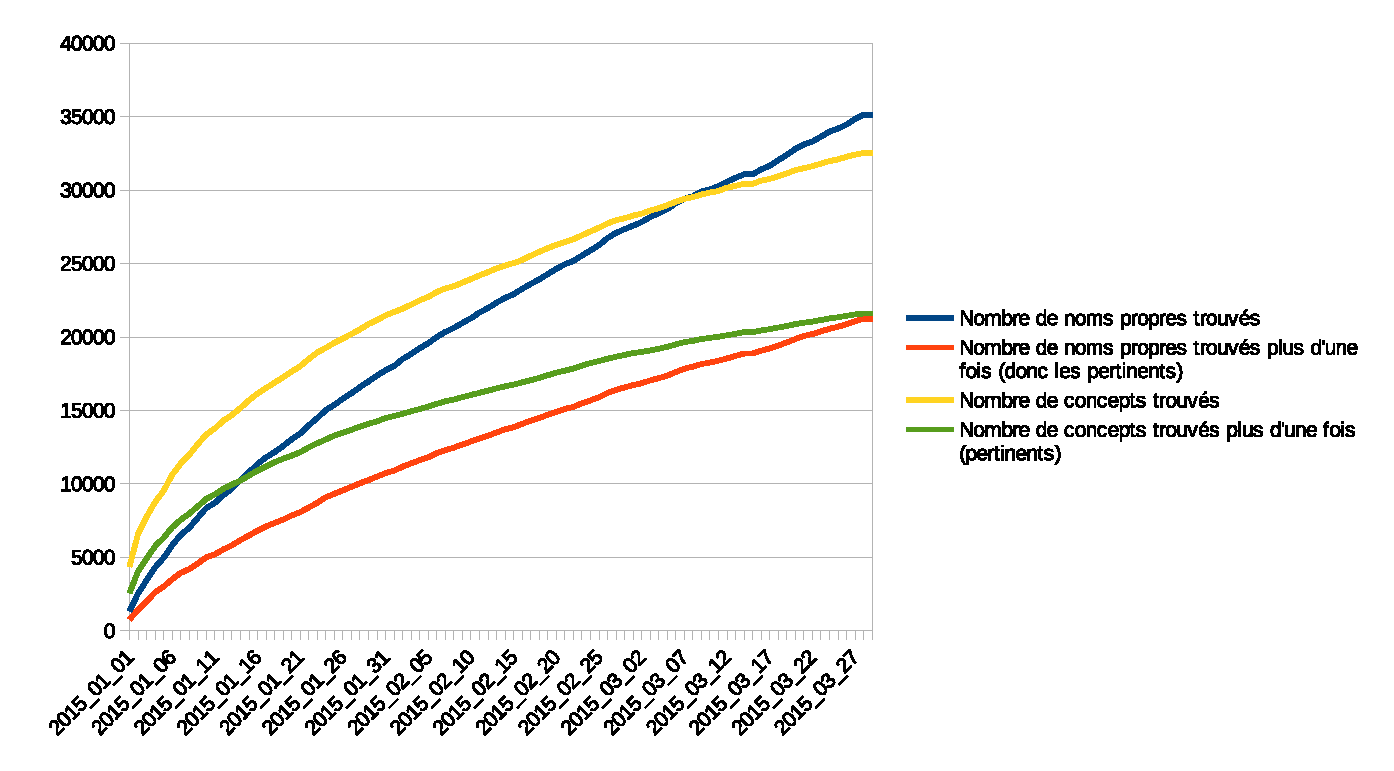
\includegraphics[width=16cm]{./conceptsnoms.eps}
 % conceptsnoms.eps: 0x0 pixel, 300dpi, 0.00x0.00 cm, bb=0 0 653 354
 \caption{\label{fig:conceptsnoms}Évolution en fonction du temps du nombre total de concepts et de noms propres tirés des articles}
\end{figure}



\subsection{WordNet}\label{Subsection:WordNet}

WordNet est une base de données lexicale pour l'anglais, produite par l'université de Princeton.

Nous l'utilisons à travers son interface \pyt{nltk}, pour récupérer des informations sur les mots et les mettre sous forme normale.


\subsection{Conceptnet5}\label{Subsection:Conceptnet5}

Conceptnet (\href{http://conceptnet5.media.mit.edu/}{leur site}) est un projet libre de graphe sémantique représentant des connaissances générales dans un spectre de domaines plutôt large. Il fait partie du \ang{Commonsense Computing Initiative} qui relie différents laboratoires, dont le MIT Media Lab, et entreprises.

Il est important de noter que Conceptnet5\index{Concepnet5} est généré à partir de données brutes. Conceptnet5 est relié à DBPedia, une grande partie de ses connaissances provient de Wiktionary, une partie de WordNet.

Nous avons utilisé une partie de code source provenant de \href{https://github.com/commonsense/conceptnet5}{<github>}.


\subsubsection{Structure de Conceptnet5}

Conceptnet5\index{Conceptnet5} est un graphe sémantique\index{Graphe sémantique} un million d'arêtes, à un ordre de grandeur près.

Les n\oe{}uds sont des mots ou de courtes phrases, dans des langues variées. Les arêtes qui relient ces n\oe{}uds expriment une connaissance, elles contiennent chacune une relation particulière.
%% Recheck
Une arête possède aussi une source (d'où provient l'information) et un poids en fonction de cette source qui quantifie l'importance de l'arête et la fiabilité de l'information apportée.

Une relation concept-arête-concept exprime une assertion\index{Assertion}. Une même assertion peut être exprimée de différentes manières. Conceptnet5 contient 1,6 million d'assertions.

Une assertion peut elle-même être utilisée comme un n\oe{}ud ou comme une arête (on peut avoir des assertions d'assertions).

Les relations valables dans tout langage, pour Conceptnet5, sont par exemple~:
\begin{itemize}
 \item RelatedTo~;
 \item IsA~;
 \item PartOf~;
 \item MemberOf~;
 \item HasA~;
 \item TranslationOf~;
 \item DefinedAs\ldots{}
\end{itemize}

Mais il en existe beaucoup d'autres.

Comme Conceptnet est construit en partie à l'aide de WordNet, il existe une correspondance entre relations de l'un et de l'autre. Par exemple~:
\begin{itemize}
 \item attribute~: Attribute~;
 \item causes~: Causes~;
 \item classifiedByRegion~: HasContext~;
 \item hyponymOf~: IsA~;
 \item sameVerbGroupAs~: SimilarTo~;
 \item seeAlso~: RelatedTo.
\end{itemize}

Cette structure étant assez proche du réseau de concepts que nous voulions construire, nous avons choisi de conserver un sous-ensemble des relations présentes dans Conceptnet qui nous on paru le plus pertinentes.

\subsubsection{Détail de l'API (\ang{Application's Programmer Interface})}

L'interface de Conceptnet5 nous autorise à faire un certain nombre de requêtes, de trois types~:
\begin{itemize}
 \item \texttt{Lookup}~;
 \item \texttt{Association}~;
 \item \texttt{Search}~;
\end{itemize}
\texttt{Association} permet de calculer la proximité entre deux concepts, ou de récupérer une liste de concepts proches d'un concept donné.

\texttt{Search} permet de récupérer une liste d'arêtes (\ang{edges}), donc de relations, entre concepts, selon les paramètres spécifiés (le plus souvent, on impose le concept de départ \ang{start} ou d'arrivée \ang{end}).

\texttt{Lookup} permet d'analyser un concept (on aura par exemple accès à des listes d'arêtes dans lequel il intervient).


\subsubsection{Utilisation de Conceptnet5}

Nous utilisons en majorité \texttt{LookUp} et \texttt{Search}, les requêtes \texttt{Association} étant beaucoup plus lentes et ne pouvant être réalisées en temps raisonnable lorsqu'il s'agit d'en réaliser plusieurs milliers.

%% Pas tout compris à ce bout
Considérons un concept dont nous cherchons des voisins dans le réseau.
\begin{itemize}
 \item On utilise une requête \verb|LookUp|\index{LookUp} pour avoir une première idée de ces voisins (une liste de liens entrant et sortants auxquels il appartient)~;
 \item Une recherche \verb|Search|\index{Search} précise pourra nous donner par exemple un certain nombre de voisins, par des liens sortants (en sélectionnant bien sûr dans ce résultat brut les concepts jugés pertinents, selon quelques critères empiriques) ;
 \item Une requête \verb|Association|\index{Association} renvoie une liste de concepts jugés similaires. On peut alors les relier au précédent avec un lien \verb|SimilarTo|.
\end{itemize}

\paragraph{Pertinence des concepts}
Conceptnet5 contient beaucoup d'informations et les concepts sur lesquels il nous aiguille ne sont pas toujours pertinents. De bons indices de la valeur d'un lien sont son poids, la nature de la relation qui l'étiquette (un lien étiqueté \verb|RelatedTo|, par exemple, pointe souvent vers la traduction du mot dans une autre langue), ou la longueur du terme vers lequel le lien pointe (il arrive que ces concepts soient une phrase entière, faisant référence à un événement extrêmement particulier, qu'on ne peut donc pas s'attendre à retrouver telle quelle dans un texte et qu'on risque de ne pas apercevoir de toute façon s'il s'y trouve).


\subsection{Freebase}\label{Subsection:Freebase}

Freebase\index{Freebase}, de même que Conceptnet, est une base de données sémantiques. Elle est cependant beaucoup plus orientées vers les noms propres, et apporte donc un nombre conséquent d'informations sur les personnes, lieux... Que l'on peut rencontrer dans les textes. Le projet, repris par Google sous une licence qui laisse les données libres d'accès, de téléchargement et d'utilisation, a lui aussi une API, un peu plus complexe que celle de Conceptnet5. Freebase permet notamment de récupérer des informations sur une personne à partir de son nom, et surtout à peu de frais, de vérifier que cette personne existe bel et bien.
%% Pas touché à ça, peut-être expliciter "complexe" ?

\section{Réseau de concepts}\label{Section:RC}


\subsection{Cahier des charges}

Le réseau de concepts\index{Réseau de concepts} est la ``mémoire à long terme'' de notre programme. L'objectif est de disposer d'une représentation souple (sous forme de graphe sémantique) de données conceptuelles qui puissent ensuite être utilisées à mieux comprendre le texte lu.

Étant donné un concept (par exemple \verb|Wayne Rooney|), à quels autres concepts est-il relié et par quelles relations~? Il est essentiel, lorsque le texte ne contient pas suffisamment d'informations ou qu'elles ne sont pas exploitables (on n'a pas toujours ``vu'' à la lecture que Wayne Rooney était un nom propre ou un humain, par exemple), d'insérer ce type de données au cœur du processus de lecture. C'est pourquoi nous avons besoin du réseau de concepts.

D'autre part, nous pouvons exiger du résumé qu'il contienne une information explicite que le texte avait sous-entendu~; par exemple, que Wayne Rooney est un joueur de football. Le réseau devra donc contenir \verb|Wayne Rooney -> isA -> Soccer player|.

Ses prérogatives ont évolué au cours de notre projet. Au début, nous pensions faire reposer une plus grande partie de l'activité de résumé du texte sur lui (notamment par le processus d'activation et le repérage des nœuds activés), alors que celle-ci s'est dirigée ensuite sur le Workspace\index{Workspace} (section \ref{Section:Traitement}).


\subsection{Structure du réseau de concepts}

\begin{definition}[Réseau de concepts]
Ce réseau est au carrefour entre les réseaux sémantiques\index{Graphe sémantique} et les réseaux de neurones. Les nœuds du réseau peuvent être vus comme représentant les concepts\index{Concept}.
\end{definition}

%%reprise textuelle
Le Réseau est constitué de n\oe{}uds. Chaque n\oe{}ud comporte~:
\begin{itemize}
  \item Une étiquette (mot) nommée concept\index{Concept}~;
 \item Une importance conceptuelle (ic) ou profondeur conceptuelle\index{Importance conceptuelle}~;
 \item Une activation (a)\index{Activation} initialement nulle~;
 \item Un certain nombre de liens à d'autres n\oe{}uds.
\end{itemize}

Chaque lien comporte~:
\begin{itemize}
 \item Une proximité conceptuelle\index{Proximité conceptuelle} (ou poids w)~;
 \item Une relation\index{Relation} qui le caractérise, prise sur le modèle de Conceptnet5\index{Conceptnet5}.
\end{itemize}

Ces différentes données numériques (proximité conceptuelle, activation, importance conceptuelle) sont normalisées entre $0$ et $100$.

\begin{figure}[h]
 \centering
 \includegraphics[width=14cm]{./rc_exemple.png}
 % rc_exemple.png: 812x612 pixel, 100dpi, 20.62x15.54 cm, bb=0 0 585 441
 \caption{\label{fig:rc_exemple}Exemple de réseau de concepts}
\end{figure}

\paragraph{}
Sur l'exemple de la figure~\ref{fig:rc_exemple}, nous revoyons les données qui nous intéressent. Les relations entre concepts sont exprimées de manière intuitive (\textit{Wayne Rooney IsA soccer player}, \textit{a soccer player is capableOf winning a match}). Nous ne représentons pas ici les poids, mais de manière générale ils favorisent la précision~: nous attendons d'eux qu'ils rendent compte du fait que si Wayne Rooney est effectivement un \textit{athlete}, il est plus pertinent de dire de lui qu'il est un \textit{soccer player}.


\subsection{Propagation d'activation}

\subsubsection{Principe}

Le réseau de concepts est dynamique. Il évolue au cours de la lecture du texte, notamment par un processus d'activation des n\oe{}uds. L'écoulement du temps est donc une donnée importante.

L'activation d'un mot (provoquée par exemple par sa lecture dans un texte) est propagée à tous les n\oe{}uds voisins. Elle permet intuitivement de penser à de nouvelles idées, de compléter l'information du texte si celle-ci est parcellaire.

Sur l'exemple de la figure~\ref{fig:rc_exemple}, l'activation du concept \verb|wayne_rooney| va provoquer dans un premier temps celle de \verb|soccer_player|, \verb|athlete|, mais aussi \verb|play_sport|, \verb|win_match|, etc.\\

La propagation d'activation doit tenir compte de plusieurs facteurs~: les poids des liens et l'importance conceptuelle des n\oe{}uds. Ainsi, un n\oe{}ud fortement relié à \verb|wayne_rooney| devra être activé plus rapidement et de façon plus importante.\\

Selon la manière dont nous voulons utiliser le réseau, il y a deux possibilités~:
\begin{itemize}
  \item Ou bien introduire un facteur de désactivation des n\oe{}uds au cours du temps, permettant éventuellement d'arriver à un état d'équilibre~;
 \item Ou bien rester en situation potentielle de déséquilibre (l'activation de chaque n\oe{}ud de la composante connexe ne cesse d'augmenter).
\end{itemize}

La notion de désactivation est assez satisfaisante intuitivement~; il existe en effet des concepts fortement activés mais peu importants, que l'on espère oublier assez rapidement. 

\subsubsection{Formalisation}
Formellement, nous utilisons les formules suivantes, inspirées de \cite{parmentier_specification_1998}.

\begin{itemize}
  \item Pour l'activation du n\oe{}ud $n$ à l'instant $t+1$~:
\begin{align}
 A_n^{t+1} = A_n^t + D^t + A^t
\end{align}
\item Pour la réactivation de ce n\oe{}ud~:
\begin{align}
 A^t = \sum_{(n' \rightarrow n \text{\ arcs entrants})} W_{(n'\rightarrow  n)} \times A_{n'}^t / 100
\end{align}
\item Pour la désactivation de ce n\oe{}ud~:
\begin{align}
 D^t = A^t \frac{100- IC_n}{100}
\end{align}
Où les facteurs $100$ sont dus à la normalisation. Si le concept a une très grande importance ($IC_n = 100$), il tend donc à ne pas être désactivé du tout. S'il a une importance très faible ($IC_n \rightarrow 0$), il a une tendance à se désactiver très rapidement.
\end{itemize}

\paragraph{}
Nous avons mis un temps plus important que prévu à extraire des importances conceptuelles véritablement utiles, et n'avons donc que peu utilisé la désactivation (qui repose sur l'importance conceptuelle). Ces importances conceptuelles ont été finalement calculées en nous inspirant de l'indice TF-IDF\index{TF-IDF}~; ce sera développé dans la partie~\ref{Section:TFIDF}.

\subsubsection{Facteur logarithmique}
Dans \cite{parmentier_specification_1998}, il était déjà question d'un facteur supplémentaire qui permette de tenir compte de la suractivation de n\oe{}uds fortement reliés. Effectivement, en l'absence de ce facteur supplémentaire, on remarque que des n\oe{}uds peu utiles mais fortement reliés (des mots et concepts courants comme \verb|person|, \verb|love|) vont rapidement être saturés, et dépasser les n\oe{}uds initiaux qui ont eux une grande importance.

Nous avons introduit ce facteur, et l'avons heuristiquement adapté. La formule d'activation d'un n\oe{}ud $n$ devient donc :
\begin{align}
 A_n^{t+1} = A_n^t + D^t + \frac{A^t}{divlog}
\end{align}
Où $divlog = \frac{\log(13 + \text{nombre d'arcs entrants})}{\log(13)}$.

Cela a donné des résultats très pertinents.

\subsubsection{Exemple}

Sur notre dernier et meilleur réseau de concepts, nous essayons par exemple d'activer simultanément deux concepts (\verb|wayne_rooney|, \verb|steven_gerrard|) et de propager cette activation :
\begin{itemize}
 \item Une fois :
 \begin{verbatim}
soccer_midfielder : 3
wayne_rooney : 60
athlete : 15
steven_gerrard : 60
person : 6
soccer_player : 15
 \end{verbatim}
 \item Deux fois, en oubliant les n\oe{}uds trop faiblement activés ($ < 5$) :
 \begin{verbatim}
  at_soccer_game : 6
wayne_rooney : 60
soccer_player : 12
break_record : 13
play_sport : 12
sport_event : 7
win_match : 6
head_ball : 9
steven_gerrard : 60
sprint : 9
jump_high : 13
athlete : 28
 \end{verbatim}
\item Quatre fois, en oubliant encore les n\oe{}uds trop faibles ($ < 10$) :
\begin{verbatim}
 sport_event : 13
player : 12
steven_gerrard : 60
athlete : 49
jump_high : 19
play_sport : 18
competition : 19
wayne_rooney : 60
sprint : 35
win : 21
break_record : 20
soccer_player : 10
\end{verbatim}
\end{itemize}
Nous pourrions aller plus loin, mais cela nous menacerait d'arriver à des n\oe{}uds fortement éloignés des deux sportifs initialement sélectionnés, et qui s'activeraient entre eux.


\subsection{Construction du réseau}
Comme cela a déjà été souligné plus haut, nous nous limitons au domaine du sport, domaine balayé par les articles qui constituent notre première source de données. 

La construction du réseau se déroule en différentes étapes, qui font intervenir quasiment toutes les sources de données de notre projet.


\paragraph{}
Certaines informations sur les éléments du réseau (poids des liens entre concepts notamment) sont relativement faciles à extraire des bases de données utilisées (Freebase, Conceptnet5 comportent déjà de telles informations, qu'il faut simplement renormaliser). En revanche, la seule manière probante d'obtenir une importance conceptuelle est de la calculer nous-mêmes.

Le réseau comporte à la fois des noms propres et des noms communs, des adjectifs, des verbes à l'infinitif~; des termes tout à fait courants (et qui ne sont pas inhérents au sport), comme des termes spécialisés.



\paragraph{Récupération de concepts et de noms}

Nous analysons un certain nombre d'articles, ici 17~000 issus de 7 flux rss différents sur 89 jours (quasiment l'intégralité des données de notre projet).


Nous avons écrit des \ang{tokenizers} adaptés aux contraintes techniques et erreurs d'écriture des données récupérées, qui viennent compléter ceux fournis par \pyt{nltk}.

Pour récupérer les noms propres, nous repérons à l'intérieur d'un article les mots marqués comme noms propres par le POS-tagger\index{Part-of-speech tagger} de \pyt{nltk}. Puis nous concaténons deux noms propres successifs. Enfin, nous retirons de la liste des noms propres ceux qui sont contenus à l'intérieur d'autres. Cette étape, largement sous-estimée au début, est cruciale puisqu'elle évite de considérer ``< nom + prénom >'' et ``<prénom>'' comme deux personnes différentes.

Nous comptons aussi la fréquence d'apparition de chaque nom et de chaque concept. 
On obtient 32~702 concepts et 35~488 noms. En réalité, un tiers d'entre eux sont des mots qui n'apparaissent qu'une seule fois, contenant par exemple des fautes d'orthographe, des néologismes ou résultant d'erreurs de notre part. On obtient par exemple~:
\begin{verbatim}
["aaron cresswell", 78]
["aaron creswell", 1]
\end{verbatim}
Ce qui suggère que dans l'un des articles trouvés, quelqu'un a commis une erreur sur le nom \verb|cresswell|. Nous éliminons donc les mots qui n'apparaissent qu'une fois. Cela nous laisse 27~070 concepts.

\paragraph{Traitement des noms avec Freebase}

Nous n'utilisons l'API Freebase que de fa\c{c}on assez simple. Chaque nom propre donne lieu à une requête. Si celle-ci aboutit, on analyse le résultat et si celui-ci comporte une donnée (exemple~: à l'envoi de \verb|"scott_jamieson"|, on récupère \verb|"soccer_midfielder"|), on ajoute un nouveau n\oe{}ud correspondant au réseau, et une arête \verb|IsA| dont le poids dépend du résultat de la requête.

L'importance conceptuelle d'un nom propre est prise par défaut comme importante.

\paragraph{Traitement des concepts avec Conceptnet5}

Chaque nouveau concept donne lieu à une requête de type \verb|Lookup|. Nous sélectionnons parmi les résultats les informations les plus pertinentes (en terme de poids, mais aussi en fonction des relations, que nous ne gardons pas toutes~: par exemple, \verb|RelatedTo| n'est pas une relation très pertinente, alors que \verb|IsA| est souvent pertinente).

L'importance conceptuelle allouée à un nouveau n\oe{}ud dépend pour beaucoup de sa fréquence d'apparition dans les articles.


\paragraph{Extension des nœuds du réseau}

Pour étendre les n\oe{}uds du réseau, nous sommes souvent amenés à chercher des liens partant d'un n\oe{}ud donné. Cela est effectué avec des recherches \verb|Search|. Nous pouvons aussi effectuer des requêtes \verb|Association| (bien que beaucoup plus lentes) afin d'induire de nouveaux liens avec des concepts similaires.



\paragraph{Suppression des nœuds inutiles}

Malgré les nombreux paramètres servant à filtrer, les requêtes n'ont pas donné des résultats toujours pertinents. Il arrive en effet qu'un terme donné (disons, \ang{captain}) soit fortement relié à deux termes n'ayant aucun rapport entre eux (ici, \ang{team} et \ang{spaceship}). Les deux liens sont très raisonnables dans l'absolu mais le second pointe vers un concept qui n'est absolument pas relié au contexte sportif~: ce genre de concepts sera isolé du reste du graphe. Nous décidons donc, pour garder un réseau aussi centré que possible sur le contexte étudié, de supprimer les concepts qui n'ont qu'un lien dans le réseau.


\subsection{Exemple de réseau de concepts}

Nous avons eu l'occasion d'effectuer différents essais de construction du réseau de concepts et nous présenterons dans cette sous-section le dernier, qui a donné les résultats les plus intéressants.

\paragraph{Étape 1~: noms propres}

\begin{itemize}
 \item Les requêtes Freebase liées aux noms propres créent 10~405 n\oe{}uds dans le réseau, ainsi que 8~255 arêtes.
 \item On lance immédiatement des requêtes Search correspondant à tous les n\oe{}uds du réseau sur Conceptnet5, afin d'acquérir plus d'informations~: on passe alors à 14~103 n\oe{}uds et 28~393 arêtes.
\end{itemize}

\paragraph{Étape 2~: concepts}

\begin{itemize}
 \item On lance une requête Lookup sur chaque concept trouvé dans les articles (27~070, les noms propres ont déjà été traités)~; on passe alors à 35~780 n\oe{}uds et 56~942 arêtes. Pour le moment, 18~762 n\oe{}uds sont certains d'être conservés (ce sont des résultats primaires de requêtes positives).
\end{itemize}


\paragraph{Étape 3~: Extension et élagage du réseau}

\begin{itemize}
 \item On étend alors l'ensemble des n\oe{}uds encore litigieux (17~018), en essayant de créer des liens vers des n\oe{}uds déjà existants, augmentant ainsi la connectivité du réseau. On passe à 76~497 arêtes.
 \item On regarde quels n\oe{}uds sont bien reliés à leur voisins, après cette opération. Au total, 28~583 n\oe{}uds semblent prometteurs.
 \item On supprime les autres n\oe{}uds. On obtient un réseau avec 28~583 n\oe{}uds et 69~307 arêtes.
\end{itemize}


\paragraph{Données quantitatives sur le réseau obtenu}

Chaque n\oe{}ud, ou concept, comporte en moyenne $2,4$ liens entrants et autant de liens sortants, ce qui suggère que les concepts sont bien reliés entre eux. On peut affiner cette observation (figures \ref{fig:liens_entrants} et \ref{fig:liens_sortants}).

\begin{figure}[h]
 \centering
% 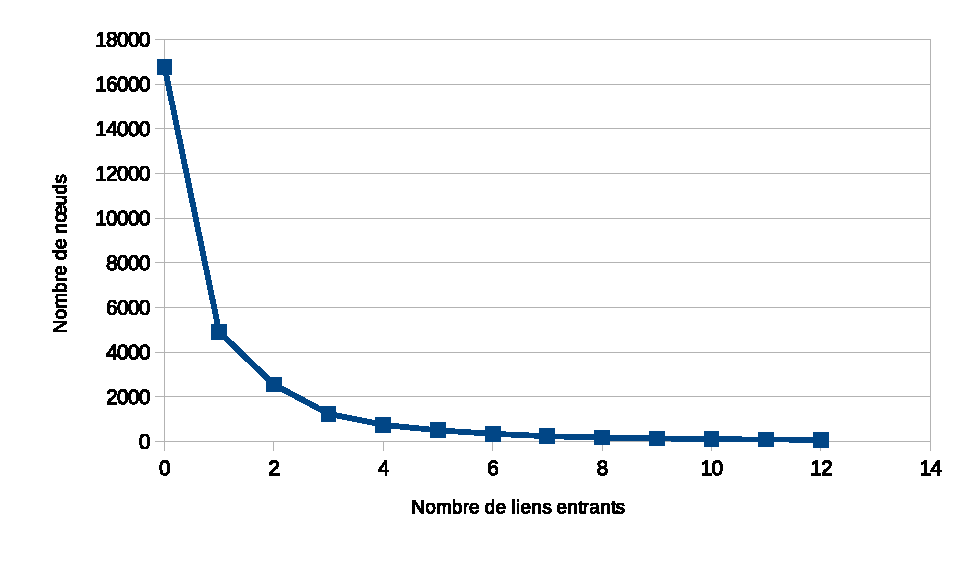
\includegraphics[width=12cm]{./liens_entrants.eps}
 % liens_entrants.eps: 0x0 pixel, 300dpi, 0.00x0.00 cm, bb=0 0 453 255
 \caption{Nombre de n\oe{}uds en fonction du nombre de liens entrants qu'ils comportent}
 \label{fig:liens_entrants}
\end{figure}


\begin{figure}[h]
 \centering
% 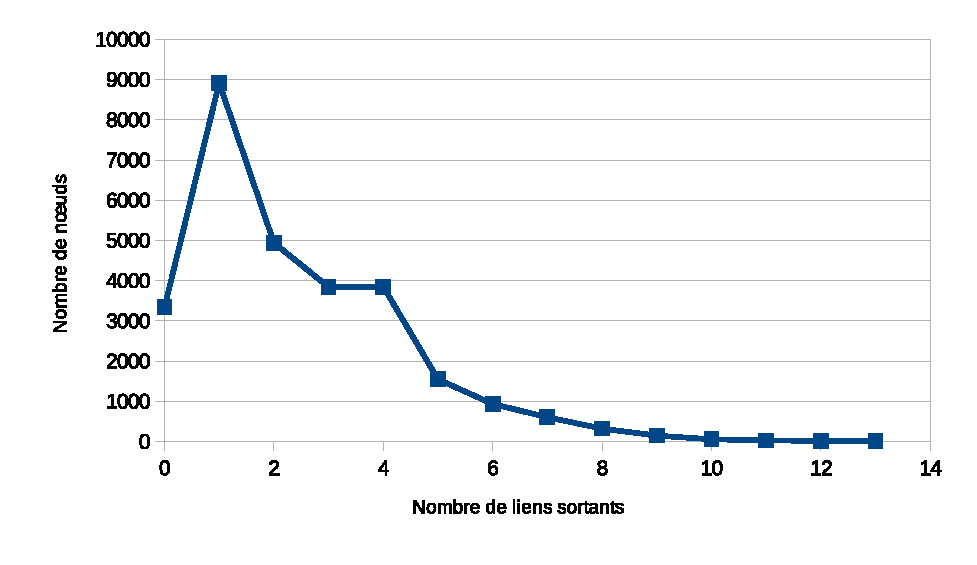
\includegraphics[width=12cm]{./liens_sortants.eps}
 % liens_entrants.eps: 0x0 pixel, 300dpi, 0.00x0.00 cm, bb=0 0 453 255
 \caption{Nombre de n\oe{}uds en fonction du nombre de liens sortants qu'ils comportent}
 \label{fig:liens_sortants}
\end{figure}

Remarquons par exemple que de très nombreux n\oe{}uds n'ont aucun lien entrant, plus de 16~000. Il s'agit en fait de concepts insérés dans le réseau au début de sa construction et qui n'ont pas ``trouvé'' de prédécesseurs lors des étapes suivantes. Ce n'est pas un défaut majeur. Ces concepts ont été trouvés dans nos textes de départ et l'on s'attend à les retrouver tels quels dans d'autres textes. Le plus important, d'obtenir une information en \textit{partant} de ces concepts, est acquis puisqu'ils possèdent des arcs sortants. En revanche, ils ne seront pas activés si on ne les trouve pas dans un texte.


\subsection{Choix de programmation du réseau de concepts}

Le réseau est enregistré sous forme de JSON Stream\index{JSON Stream}, un type de données repris à Conceptnet5, qui permet sans contrainte technique majeure de l'écrire sous forme facilement lisible par un utilisateur extérieur. Il s'agit tout simplement d'une liste d'objets Python pouvant être transformés en JSON (typiquement, n\oe{}uds et arêtes du graphe), écrits l'un après l'autre, ligne par ligne dans un fichier.\\

Le stade suivant consisterait bien sûr à utiliser une base de données pour stocker et traiter le réseau, mais le nombre de n\oe{}uds étant resté raisonnable, nous n'avons pas eu à abandonner le package \pyt{networkx} qui nous permet de le représenter en mémoire sous forme de graphe.

\paragraph{}
Nous avons parallélisé les requêtes afin de les effectuer dans un temps raisonnable, même si l'opération de construction du réseau (sa version à 30~000 n\oe{}uds) reste longue dans son ensemble (plus d'une heure) et que les quantités de données mises en jeu suggèrent qu'une utilisation différente, notamment de Conceptnet5 (téléchargement et recherche dans la base de données de façon locale), pourrait être faite.



\section{Méthodes statistiques avec TF-IDF}\label{Section:TFIDF}

La méthode statistique consiste à extraire des phrases par des techniques de la fouille de données textuelles. L'idée principale est de pondérer les phrases selon leur représentativité dans le texte et d'afficher celles de poids le plus fort dans l'ordre de leur apparition dans le texte et dans la limite de la taille du résumé. Nous avons choisi ici l'indice TF-IDF pour mesurer ces poids.

\subsection{Algorithme statistique}

Pour donner à chaque phrase un poids, on cherche d'abord à mesurer l'importance de chaque mot. On a observé qu'il y a des mots qui se présentent presque dans tous les documents comme les articles, les auxiliaires, etc. Il faut donc filtrer ces mots non-significatifs. D'autre part, les mots-clés d'un texte sont aussi des mots qui y sont fréquents et à qui doit donc être assigné un poids important.

On cherche donc ici un indice qui diminue selon le nombre d'apparitions dans tous les documents, et qui augmente selon le nombre d'apparitions dans le texte particulier. Et l'indice TF-IDF satisfait exactement ces critères.


\subsection{TF-IDF pour le résumé automatique}
Selon une lemme de Hans \textsc{Peter Luhn}, le poids d'un terme est proportionnel à sa fréquence.

D'après la loi de \textsc{Zipf}, la fréquence d'occurrence $f(n)$ d'un mot est liée à son rang $n$ dans l'ordre des fréquences par une loi de la forme $f(n) = \frac{K}{n} $ où K est une constante.

%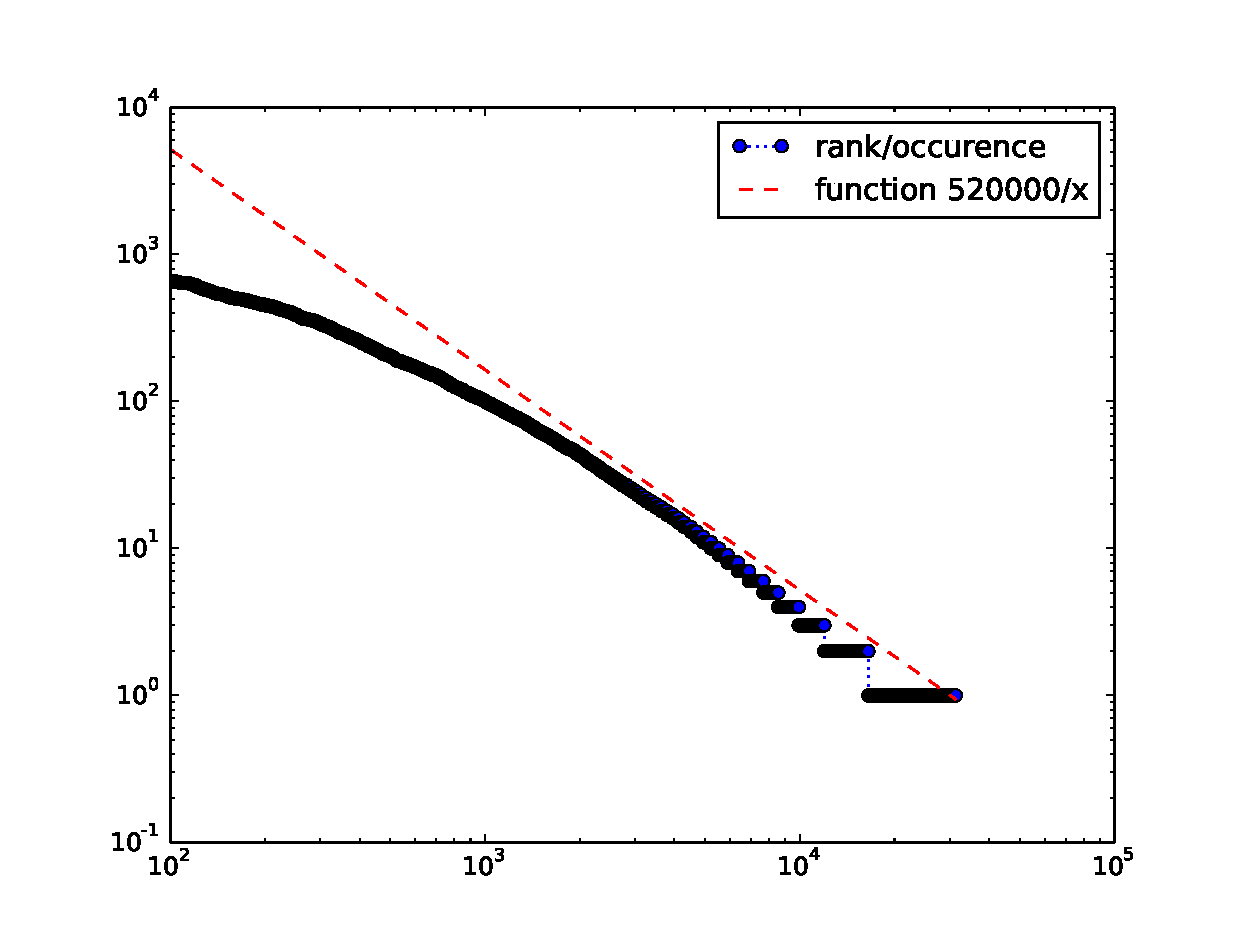
\includegraphics[scale=0.5]{loi_de_zipf.eps}

L'abscisse x est le rang d'un terme selon la fréquence et y est l'occurrence de ce terme. Les mots plus fréquents sont 'the','of' et 'and'. On voit bien que la courbe tend vers la fonction $K/x$.(ici on a choisi K = 5200000) C'est-à-dire que pour chercher les mots indiscriminants, il suffit de regarder l'inverse de la fréquence d'occurrence.

\subsubsection{Définition formelle}

\begin{definition}[TF]
 La fréquence d'un terme (\textit{term frequency}, TF) que l'on mesure ici est juste le nombre d'occurrences de ce terme dans le document considéré.
\end{definition}

\begin{definition}[IDF]
 La fréquence inverse de document (\textit{inverse document frequency}, IDF) est une mesure de l'importance du terme dans l'ensemble du corpus. Elle vise à donner un poids plus important aux termes les moins fréquents, considérés comme plus discriminants.
\end{definition}

Ici, on prend le logarithme de cette fraction~:

\begin{align}
 IDF_{i} =  log \frac{|D|}{|\{d_{j}: t_{i} \in d_{j}\}|}
\end{align}

Où : 
\begin{itemize}
 \item |D| est le nombre total de documents dans le corpus ;
 \item $|\{d_{j} : t_{i} \in d_{j}\}|$ est le nombre de documents où le terme  $t_{i}$  apparaît (c'est-à-dire  $n_{i,j} \neq 0$)
\end{itemize}

Plus un mot apparaît, plus son indice IDF est proche de zéro. Des mots qui sont présents dans tous les documents vont notamment être filtrés car ils ont un indice nul.

\begin{definition}[TF-IDF]
Le poids du mot s'obtient en multipliant les deux mesures TF et IDF.
\end{definition}

\begin{align}
 TFIDF_{i,j} = TF_{i,j} \cdot  IDF_{i}
\end{align}

\begin{definition}[Poids d'une phrase]
Après avoir calculé les indices TF-IDF de chaque mot dans une phrase, on les somme et divise cette somme par le nombre de mots dans cette phrase : c'est le poids de cette phrase (on oubliera bien sûr les phrases trop courtes, moins de deux concepts, pour lesquelles le poids peut être défini comme nul).
\end{definition}

\subsubsection{Illustration}
Voyez le tableau de valeur TF-IDF de 4 termes dans 3 documents sur un corpus de 1000 documents.
\begin{center}
	\begin{tabular}{|c|c|c|c|c|}
	 \hline
	 	Terme & TF(document 1) & TF(document 2) & TF(document 3) & IDF \\
	 \hline
	 	he & 90 & 61 & 63 & 0.006 \\
	 \hline
	 	on & 43 & 34 & 51 & 0.008 \\
	 \hline
	 	discussion & 11 & 0 & 0 & 6.39 \\
	 \hline
	 	traveller & 0 & 13 & 0 & 6.39 \\
	 \hline
	\end{tabular}
\end{center}

Et les TF-IDF de ces 4 termes se calculent comme ci-dessous:

\begin{center}
	\begin{tabular}{|c|c|c|c|}
	 \hline
	 	Terme & TF-IDF(document 1) & TF-IDF(document 2) & TF-IDF(document 3) \\
	 \hline
	 	he & 0.540 & 0.366 & 0.378 \\
	 \hline
	 	on & 0.344 & 0.272 & 0.408 \\
	 \hline
	 	discussion & 70.29 & 0 & 0 \\
	 \hline
	 	traveller & 0 & 83.07 & 0 \\
	 \hline
	\end{tabular}
\end{center}

On voit ici l'influence de la fréquence inverse sur le TF-IDF: dans le document 1, même si le terme 'he' est plus fréquent que celui de 'dicussion', son indice TF-IDF est petit, car il apparaît dans la plupart des documents et a un indice IDF petit. Pour le document 1, 'discussion' est plus discriminant que 'he'.

\paragraph{}
Après avoir obtenu les valeurs TF-IDF de chaque terme, on peut calculer les poids de chaque phrase. Notre résumé est construit en additionnant la première phrase du texte (souvent le titre, qui, riche en information, a souvent le meilleur poids) avec quelques autres ayant un poids maximal, prises dans leur ordre d'apparition dans le texte.

On peut ainsi facilement agir sur la longueur du résumé par rapport à celle du texte (ne sélectionner qu'une phrase sur trois, ou sur quatre).

\subsection{Tests et qualité des résumés obtenus}

Même que la méthode TF-IDF est efficace pour la recherche de mot clé, la qualité des résumés obtenus est peu optimale. En effet, avec un regroupement simple de phrases, on perd beaucoup d'information contextuelle. Par exemple, on peut avoir souvent une phrase commençant par un mystérieux \textit{he} (il) ou \textit{she} (elle). Et cette phrase sans contexte est souvent peu compréhensible. (C'est aussi pour cela que nous choisissons d'inclure dans le résumé la première phrase, car elle contient \textit{a minima} les noms des personnes dont l'article traite).

Deux exemples sont disponibles en annexe \ref{Annexe:resumes}.


\subsection{TF-IDF pour l'importance conceptuelle}

Dans un premier temps, l'importance conceptuelle\index{Importance conceptuelle} n'était définie que de manière floue et n'était pas dérivée d'informations quantitatives autres que des fréquences d'apparition de concepts (des concepts apparaissant plus souvent étant favorisés).

Nous avons donc adapté l'indice TF-IDF pour calculer une importance conceptuelle. Cela a même pu être adapté aux noms propres.

L'idée est que les termes ayant une importance conceptuelle forte sont ceux qui~:
\begin{itemize}
 \item Ont une fréquence (TF) élevée ;
 \item Et un IDF fort, c'est-à-dire qu'on les trouve rarement dans l'ensemble du corpus.
\end{itemize}

La différence avec le calcul précédent de TF-IDF est que le TF était calculé de manière locale à un document, alors qu'ici, il est calculé de manière globale, étant donné que nous ne nous positionnons pas sur un document en particulier.

\paragraph{}
Ce calcul est effectué d'une part sur les noms propres, d'autre part sur les concepts (nous n'avons pas cessé depuis le début de séparer les uns et les autres). L'intérêt reste toujours le même : pour les noms propres, cela va rendre compte de l'importance qu'a chaque personne. De manière générale, les TF globaux des concepts sont beaucoup plus importants que ceux des noms propres, et les IDF sont beaucoup plus faibles : lorsqu'il apparaît, un nom propre apparaît moins fréquemment et dans un moins grand nombre de documents.

Le résultat est un TF-IDF très important pour certains concepts, même par rapport aux meilleurs noms, nous faisant conclure qu'une renormalisation différente (pour transformer en un indice entre 0 et 100) pour les deux catégories sera nécessaire.

\paragraph{}
Une partie représentative des résultats est reproduite en annexe \ref{Annexe:TFIDF}.

On remarque notamment, dans le cas des noms propres, que les faux noms propres (erreurs de POS-tagging) se sont retrouvés en bas du tableau. En effet, même lorsqu'ils apparaissent plusieurs fois, ce sera dans plusieurs textes distincts, alors qu'un véritable nom propre à même fréquence aura tendance à apparaître plusieurs fois dans le même document.


\section{Traitement préalable des données}

Pour assurer une certaine cohérence entre les données présentes dans le réseau de concepts et celles présentes dans le Workspace, il est bien sûr nécessaire de faire le même travail de normalisation qui a eu lieu lors de la construction du premier. Cependant, le Workspace étant destiné à contenir des informations beaucoup plus précises et ciblées sur un texte que le réseau, il est nécessaire de faire un travail préalable sur les données du texte avant des les introduire dans le Workspace. Ces étapes sont décrites ci-dessous et se regroupent en deux parties : une analyse syntaxique, d'une part, permettant d'établir les liens entre les différents éléments du texte ; et d'autre part un travail sur la reconnaissance des pronoms permettant de distinguer les différentes entités présentes dans le texte.

\subsection{Analyse syntaxique}\index{Analyse syntaxique}

Cette partie ne constituant pas le c\oe{}ur de notre PSC, nous avons décidé d'utiliser un outil déjà codé. L'entreprise Systran, au sein de laquelle notre tuteur travaille, a accepté de traiter nos données et nous a renvoyé un graphe sémantique contenant une analyse syntaxique complète des articles du corpus..

\subsubsection{Description algorithmique d'une grammaire}\index{Grammaire}
Une grammaire peut être décrite informatiquement de manière très simple. En effet, on peut la voir comme~:
\begin{itemize}
	\item Un ensemble de classes terminales (verbe, nom par exemple) associées à une liste de mots ou éventuellement d'expressions
	\item Un ensemble de règles, souvent sous la forme d'une reconnaissance de motifs, permettant de découper une phrase en plusieurs éléments (et finalement en unités syntaxiques élémentaires).
\end{itemize}

Il y a par conséquent deux manières pour une grammaire d'être incomplète~: soit elle ne connaît pas assez de vocabulaire (manque d'éléments dans les cas terminaux), soit elle ne connaît pas assez de règles. La première faille est assez facile à combler par des requêtes vers WordNet\index{WordNet} (et par ailleurs un outil automatique est inclus dans \pyt{nltk}\index{Natural Language ToolKit})~; il est en revanche assez indispensable d'avoir une grammaire complète en termes de règles car il est beaucoup plus difficile d'inventer des manières de découper une phrase.

Il est également à noter que les grammaires modernes s'appuient sur un entraînement statistique et traite les données de manière stochastique.

\subsubsection{\'Etat du texte en fin d'analyse}
Les données traitées par Systran nous sont revenues sous la forme d'un graphe sémantique. Chaque nœud, ou mot, de la phrase était de plus enrichi d'une liste de tags permettant d'établir de quel genre de mot il s'agit (humain, véhicule, lieu si c'est un nom; verbe d'action, verbe descriptif si c'est un verbe; etc.) Notons également que chaque nœud contient une liste (éventuellement vide) de fils avec lesquels il forme une entité syntaxique cohérente telle qu'un groupe nominal. Cela nous a été très utile lorsqu'il s'est agit de faire la différence entre les entités et leurs attributs lors de leur incorporation dans le Workspace.

Ces données ont ensuite été transcrites sous la forme d'une classe python appelée \pyt[GrammarTree]. 

\subsection{Résolution de pronoms}

Le but de la résolution de pronoms\index{Résolution de pronoms} est, étant donné une phrase qui peut être par exemple~:

\begin{verbatim}
 Sepp_+_Blatter is the favourite to win a Fifa race he vowed he would not stand for.
\end{verbatim}
de rapporter chaque pronom à un groupe nominal. Ici, les deux pronoms que l'on repère (``he'') se rapportent évidemment à \verb|Sepp_+_Blatter|.

Nous disposons pour nous aider des données fournies par l'analyseur syntaxique de Systran. En voici une liste non exhaustive~:
\begin{itemize}
 \item POS\index{Part-of-speech}
 \item Type grammatical de chaque mot~: nom propre, acronyme, verbe, auxiliaire, préposition\ldots{}
 \item Différents liens entre les mots~: adjectif relié à un nom, article\ldots{}
\end{itemize}


\subsubsection{Étape 1}
On commence par trouver l'ensemble des groupes nominaux. Nous avons deux choix~:
\begin{itemize}
 \item Ou bien les trouver tous~;
 \item Ou bien se limiter d'emblée à ceux qui ont leurs chances.
\end{itemize}

Nous prenons d'abord le deuxième choix~: l'analyseur de Systran nous indique en particulier, étant donné un mot, s'il est objet ou sujet d'un verbe. Nous considérons donc, dans un premier temps, que les noms concernés sont les noms principaux et que tous les groupes nominaux qui nous intéressent se construisent autour d'eux.

Après expérience, nous avons étendu le ``droit'' de créer un groupe nominal à de simples compléments d'objet, constatant qu'ils apparaissaient eux aussi.


\subsubsection{Étape 2}
On considère maintenant l'ensemble des pronoms.

Pour un pronom situé à une position donnée, les groupes nominaux\index{Groupe nominal} potentiels font l'objet d'un classement, relatif à un score, que nous calculons de la manière suivante~:

\begin{itemize}
 \item Un candidat a le droit d'être situé dans une phrase précédente (sous une limite fixée à 2 ou 3). Plus il est éloigné du pronom, plus son score diminue. S'il est après le pronom, son score diminue drastiquement (voire $-\infty$).
 \item Le candidat doit vérifier certaines correspondances avec le pronom~: en particulier, il doit avoir le même genre et le même nombre. Si c'est vérifié, le score augmente. Sinon, le score diminue. Cette information n'est pas tout le temps disponible. En revanche, on sait parfois si le groupe nominal concerné (son nom principal) est un humain ou non.
 \item On a parfois (notamment avec le pronom ``that'') de manière directe l'information de l'antécédent. L'antécédent désigné doit alors gagner un score énorme (voire $+\infty$, mais l'analyseur de Systran n'est pas infaillible).
 \item Un groupe nominal qui apparaît au début d'une phrase doit, quels que soient les pronoms, avoir un meilleur score. Les noms propres apparaissent souvent au début de la phrase pour être ensuite rappelés par des pronoms, c'est d'ailleurs le cas dans l'exemple ci-dessus.
 \item Un groupe nominal répété gagne également en score.
 \item Un groupe nominal précédé d'une préposition perd en score.
 \item Un groupe nominal sujet gagne en score, et un groupe objet perd en score. 
 \item Un groupe nominal comportant un article indéfini perd en score.
 \item Un groupe nominal comportant un nom propre gagne en score.
\end{itemize}

Ces différentes exigences satisfont à un impératif de simplicité. On cherche ensuite à balancer le mieux possible les augmentations/diminutions de score afin de maximiser la pertinence des résultats.

Nous nous inspirons pour cette méthode de \cite{Mitkov:1998:RPR:980691.980712}, pour sa simplicité et son adaptabilité quant aux données dont nous disposons.


%%%%%%%%%%%%%%%%%%%%%%%%%%%%%%%%%%%%%%%%%%%%%%%%%%%%%%%%

%%%%%%%%%%%%%%%%%%%%%%%%%%%%%%%%%%%%%%%%%%%%%%%%%%%%%%%ù

%%%%%%%%%%%%%%%%%%%%%%%%%%%%%%%%%%%%%%%%%%%%%%%%%%%%%%%ù

\section{Traitement du réseau}\label{Section:Traitement}

Le réseau de concepts représente, comme nous l'avons déjà dit, la connaissance \textit{a priori} de notre programme sur le domaine étudié. Pour étudier un texte particulier, il s'agit maintenant de faire agir ce texte sur nos connaissances et d'interpréter l'effet que cette lecture a.

Deux méthodes ont été envisagées~: la première étudiait, essentiellement, la différence entre l'état du réseau de concepts avant et après la lecture et devait en déduire les faits importants. La seconde, qui a finalement été retenue, s'appuie sur une activation des concepts dans le réseau, puis une instanciation des concepts fortement activés dans un espace de travail appelé \textit{Workspace}\index{Workspace}. Ces concepts instanciés sont par la suite capables d'effectuer des tâches plus complexes relatives à la compréhension du texte.

Quelle que soit la méthode employée, une analyse syntaxique\index{Analyse syntaxique} préalable du texte est nécessaire pour rendre compte de sa compréhension et utiliser au mieux notre réseau de connaissances.

\subsection{Workspace}\index{Workspace}
Le Workspace est une zone où on va stocker des structures formées à partir de concepts et travailler dessus. Par opposition au réseau de concepts, qui représente une connaissance relativement figée du monde, ces structures visent à représenter la compréhension que l'on a pu acquérir du texte.
Par exemple, un type de structure rencontré dans le Workspace serait un graphe décrivant l'évolution de l'état d'un objet au fur et à mesure du temps, d'après ce qu'on a pu extraire du texte.

\subsubsection{Structure du Workspace}
Comme on l'a dit il s'agit essentiellement d'une structure de graphe orienté.

Les nœuds représentent des concepts présents dans le texte à résumer ou bien des concepts qui lui sont liés. On différencie ces concepts en deux sous-classes, selon qu'il s'agit d'entités ou d'attributs.

\begin{definition}[Entité]
On parle d'entité pour désigner une chose ou une personne formant une unité, réelle ou non, capable d'agir ou de subir des actions dans le cadre du texte. Un fantôme ou une voiture sont des entités ; deux voitures forment deux entités distinctes ; et la joie (par exemple) n'est pas considérée comme une entité.
\end{definition}
\begin{definition}[Attribut]
Un attribut est un concept altérant ou complétant le sens d'un autre. Par exemple, "Angleterre" dans "l'équipe d'Angleterre" est un attribut de "l'équipe". L'attribut n'ayant pas de sens à lui seul, on parlera toujours de l'attribut de telle entité.
\end{definition}

On voit déjà sur ces exemples simples que la distinction entre entité et attribut n'est pas triviale. En effet, dans un contexte différent, l'Angleterre pourrait être considérée comme une entité. Elle est pourtant essentielle à la compréhension du texte, et donc à son résumé, dans la mesure où ce seront les entités qui seront le sujet du texte.

De plus, les structures du Workspace doivent être capables de rendre compte des actions effectuées ou subies par les entités. Pour cela, il nous a semblé plus facile d'étudier l'effet qu'ont ces actions sur l'état des entités : on parle alors d'évènement.

\begin{definition}[État]
L'état d'une entité désigne l'ensemble de ses attributs à un moment donné.
\end{definition}
\begin{definition}[Évènement]
Un événement est une arête dans le graphe présent dans le Workspace, reliant une entité ou un attribut à un autre. Si l'origine est une entité, il représentera le plus souvent une action ; si l'origine et la destination sont des attributs il représentera plutôt un changement dans l'état de l'entité à laquelle ils sont reliés.
\end{definition}

\subsubsection{Implémentation}

Pour l'implémentation, on utilise une seule classe python implémentant Networkx. Cela nous fournit une architecture agréable pour traiter les liens entre nos diverses entités et attributs (qui existent en tant que nœuds du réseau). Les évènements sont implémenté en tant qu'arêtes étiquetés du graphe.

\subsubsection{Utilisation}

Le fait d'ajouter des liens syntaxiques et logiques (par les évènements) entre les concepts intervenant dans le texte nous permet d'accéder de manière assez directe à leur importance relative dans le texte. En effet, du point de vue syntaxique, un concept fortement connecté sera présent dans une grande partie du texte et pourra donc être considéré comme le sujet, au moins du point de vue de l'auteur du texte, de ce dernier. Si, qui plus est, une entité ou ses attributs est l'origine ou la destination de nombreux évènements, il constituera un point central du texte au niveau du contenu.

Ainsi l'importance d'un concept, tant du point de vue de la forme que du fond, nous semble directement reliée à la connectivité des entités dans le graphe. Cependant, si la résolution des pronoms et des entités nous permet de repérer des références communes à une entité donnée dans le texte, la structure du workspace n'est pas adaptée à mesurer des rapprochements conceptuels entre diverses entités ou attributs. Par conséquent, nous avons décidé de nous servir des termes présents dans le workspace pour activer les concepts auxquels ils réfèrent dans le réseau de concepts, et ce d'autant plus qu'ils étaient bien connectés au reste du graphe sémantique représentant le texte source. La propagation de l'activation au sein du réseau de concepts permet alors de régulariser quelque peu l'importance des diverses entités mises en jeu, et surtout de faire les rapprochements conceptuels souhaités.

Finalement, l'algorithme complet se déroule ainsi~:
%% TODO : Recheck

\begin{enumerate}
	\item On parcourt l'arbre grammatical représentant le texte et on plonge chaque entité, attribut, et évènement rencontré dans le workspace. Au préalable, s'il y a plusieurs références à une entité donnée existent, elles sont toutes gardées et leurs attributs sont mutualisés~;
	\item Sur la base de la connectivité des différents termes présents dans le workspace, on active les concepts correspondant dans le réseau de concepts~;
	\item Les entités correspondant aux concepts les moins activés sont éliminés du workspace~;
	\item Les quelques nœuds restants sont présentés au lecteur.
\end{enumerate}

%% À vérifier
Le résultat final est alors un petit nombre d'entités centrales dont parle le sujet. Les relations verbales entre ces entités permettent au lecteur de se faire une idée raisonnable du contenu initial du texte, même si la représentation qui lui en est donnée n'est pas du langage naturel.


\section{Bilan et améliorations envisageables}

Le projet a été essentiellement mené au terme annoncé, malgré quelques changements de dernière minute qui nous ont empêché d'évaluer de manière correcte nos résultats. Dans son état actuel, nous n'avons pas exactement atteint l'objectif affiché de faire un résumé capable de s'affranchir de la formulation première du texte. Nous apportons cependant un véritable changement sur la manière d'obtenir notre résumé~: là où la plupart des algorithmes se basent sur des récurrences statistiques de termes, nous nous efforçons de reconnaître les entités et les concepts mis en jeu et de travailler sur ceux-ci.

\subsection{Considérations techniques}

Le code de notre projet, de grande taille, est entièrement documenté.

\subsection{Bilan des actions menées}

Dans son état actuel, le projet constitue une excellente préparation à la mise en place des méthodes que nous avons décrites. Nous avons en effet amélioré quelques outils de traitement de données textuelles brutes (en ce qui concerne le traitement des noms propres notamment). Nous avons également pu mettre en place les structures indispensables à nos algorithmes et créé les fonctions faisant l'interface avec les structures de données déjà existantes.

Nous avons, d'autre part, pu implémenter un algorithme raisonnable de résumé automatique s'appuyant sur TF-IDF. % Complement needed.



\vspace{1\baselineskip}

%\subsection{Améliorations}

%\subsubsection{Apprentissage du réseau de concepts}
%Le réseau de concept représente un \textit{a priori} sur le monde de notre programme. Il est donc normal que cette structure évolue au fur et à mesure des textes lus.

%Les fonctions de construction du réseau peuvent sans mal être appelées après la génération du résumé pour y apporter des modifications pérennes, que ce soit sur les données brutes ou, mieux encore, sur les structures encores présentes dans le Workspace qui contiennent explicitement des relations entre les différents concepts présents.


%\subsubsection{\'Evaluation des résumés}
%Le faible nombre de résumés que nous prévoyons de produire nous permettra d'utiliser la méthode la plus simple parmi celles qui étaient mentionnées dans la proposition détaillée~: la comparaison à un résumé déclaré bon car produit par un humain.

%L'idée est la suivante~: l'un de nous résumera un texte, nous emploierons notre programme pour résumer le même texte, et enfin nous utiliserons un simple algorithme statistique (basé sur TF-IDF) pour résumer ce même texte. Nous comparerons ensuite ces résumés du point de vue de l'information qu'ils contiennent~: sont-ils des images assez fidèles du document original~?

%Compte-tenu de la simplicité de l'algorithme statistique, nous espérons que le résumé produit par notre programme se situera quelque part entre le résumé statistique et le résumé humain.



 

\section{Références bibliographiques}

\begin{quotation}
 This work includes data from ConceptNet 5, which was compiled by the Commonsense Computing Initiative. ConceptNet 5 is freely available under the Creative Commons Attribution-ShareAlike license (CC BY SA 3.0) from http://conceptnet5.media.mit.edu. The included data was created by contributors to Commonsense Computing projects, contributors to Wikimedia projects, Games with a Purpose, Princeton University's WordNet, DBPedia, OpenCyc, and Umbel.
\end{quotation}

\nocite{*}
\printbibliography{}

\newpage
\appendix

\section{Indices TF-IDF pour certains concepts et noms propres}

Les indices reproduits ci-dessous ne sont pas normalisés.

\begin{figure}[!h]
\begin{center}
 \begin{tabular}{|c|c|}
 \hline
  \textbf{Terme} & \textbf{TF-IDF} \\
  \hline
  goal & 18036.355588902752 \\
  club & 16707.84340604437 \\
  win & 16416.987149003868 \\
  player & 15395.13561971935 \\
  do & 14983.099117885753 \\
  get & 14831.125247005852 \\
  game & 14772.460116022885 \\
  team & 14736.039158065283 \\
  season & 14410.376362720359 \\
  score & 14347.834720380053 \\
  fan & 14345.794404055676 \\
  ball & 14183.767993101164 \\
  say & 14041.53077169254 \\
  play & 13932.858353857095 \\
  go & 13866.246326872366 \\
  share & 13220.473403693579 \\
  year & 13048.180880727492 \\
  football & 12974.031162373381 \\
  time & 12476.391302456212   \\
  right & 12370.950387951321     \\
  think & 12340.221480751856   \\
  first & 12325.427075870062   \\
  watch & 12318.296129723469   \\
  last & 12292.45714341061   \\
  match & 12258.013990918109   \\
  side & 12245.076493840706   \\
  leave & 12133.864922485838   \\
 $\cdots$ & $\cdots$ \\
    kangaroo  & 9.025515684964109  \\
  q  & 8.620050576855945  \\
  wristband  & 8.620050576855945  \\
  fifteenth  & 8.620050576855945  \\
  refinance  & 8.620050576855945  \\
  wishy-washy  & 8.620050576855945  \\
  inheritance  & 8.620050576855945  \\
  annex  & 8.332368504404164  \\
  featherweight  & 8.332368504404164 \\
  \hline
 \end{tabular}
\label{fig:TFIDFConcepts}
\caption{Extrait de la base de données de TF-IDF pour des concepts}
\end{center}
\end{figure}

\newpage
\begin{figure}[h!]
\begin{center}
 \begin{tabular}{|c|c|}
 \hline
  \textbf{Nom} & \textbf{TF-IDF} \\
  \hline
  chelsea  & 15435.05496583199 \\
  premier league  & 14572.723366675536 \\
  liverpool  & 14412.6737426319 \\
  foul  & 10777.070534251237 \\
  steven gerrard  & 9402.731890649875 \\
  louis van gaal  & 9163.915519209326 \\
  cup  & 9132.154367268871 \\
  attempt  & 8675.8177744147 \\
  barcelona  & 8578.435422472256 \\
  england  & 8278.73616736681 \\
  lionel messi  & 7657.736882963432 \\
  harry kane  & 7460.74448794179 \\
  cristiano ronaldo  & 7375.310093934143 \\
  tottenham  & 7119.794079790657 \\
  burnley  & 5942.596160930355 \\
  league  & 5847.736458560602 \\
  diego costa  & 5674.059267902648 \\
  wayne rooney  & 5382.705157188505 \\
  radamel falcao  & 5141.135765623698 \\
  gareth bale  & 4761.904077325407 \\
 $\cdots$ & $\cdots$ \\
  %whet  & 9.718662865524054 \\
  %embrace  & 9.718662865524054 \\
  %oar  & 9.718662865524054 \\
  autograph  & 9.718662865524054 \\
  faith  & 9.718662865524054 \\
  attitude  & 9.718662865524054 \\
  place  & 9.025515684964109 \\
  blueprint  & 9.025515684964109 \\
  ergo  & 9.025515684964109 \\
  subscribe  & 9.025515684964109 \\
  bold  & 9.025515684964109 \\
  hear  & 9.025515684964109 \\
  thing  & 9.025515684964109 \\
  ohio  & 9.025515684964109 \\
  lanky  & 9.025515684964109 \\
  mustapha carayol  & 9.025515684964109 \\
  innocent  & 9.025515684964109 \\
  count  & 9.025515684964109 \\
  detroit  & 9.025515684964109 \\
  our  & 8.620050576855945 \\
  not  & 8.620050576855945 \\
  fenway park  & 7.926903396296 \\
  \hline
 \end{tabular}
\label{fig:TFIDFNoms}
\caption{Extrait de la base de données de TF-IDF pour des noms propres}
\end{center}
\end{figure}

\newpage

\section{Exemples de résumés avec une méthode statistique}

\subsection{Texte 1}

Tiré du site de \href{http://www.theguardian.com/football/2015/mar/29/georgia-germany-euro-2016-match-report}{\textit{The Guardian}}, le 29 mars 2015.

(Notons une erreur survenue dans la récupération de l'article : la légende de l'image a été prise comme faisant partie du texte.)\\

\begin{quotation}
\texttt{
Germany's Marco Reus,  right,  celebrates his goal against Georgia.\\
Photograph.\\
David Mdzinarishvili/ REUTERS.\\
The World Cup winners Germany eased past the hosts Georgia 2-0 in their Euro 2016 qualifier on Sunday with first-half goals from Marco Reus and Thomas Müller enough to get their Group D campaign back on track.\\
Reus put the visitors ahead after 39 minutes and Müller doubled their lead before the break as the Germans,  who had an erratic start to the qualifiers last year when they lost in Poland,  were never threatened by their weaker opponents.\\
The win lifted Germany,  who did not need to hit top form,  to 10 points from five games to equal Poland,  who take on Ireland later on Sunday,  and Scotland.\\
Georgia have had a tough start in Group D,  recording four defeats and a win in Gibraltar to stay on three points.\\
It did not take long for Germany,  with several World Cup winners back in the squad including captain Bastian Schweinsteiger,  to threaten and Reus’ powerful drive was palmed on to the crossbar by the keeper Giorgi Loria after five minutes.\\
With the coach Joachim Löw reverting to a four-man defence from a three-player experiment against Australia in a friendly on Wednesday,  Germany pressured their opponents’ box for most of the first half.\\
Müller fired at goal directly from a corner only to see the ball fly just wide of the post and Mesut Özil missed another big chance as the visitors had the hosts firmly on the backfoot.\\
Reus did better in the 39th when Mario Götze charged into the box and was lucky to scramble the ball to the winger,  who drilled home for his second goal this week after also scoring in their 2-2 friendly draw against Australia.\\
Müller then added another on the stroke of halftime to firmly put Germany in the driving seat.\\
The new Georgia coach Kakhaber Tskhadadze added a forward after the break but it was Reus who came close again,  rattling the bar for a second time on the hour with another powerful shot.\\
}
\end{quotation}

\subsection{Phrases du texte 1 par poids décroissants}

\begin{quotation}
\texttt{
 ( The win lifted Germany,  who did not need to hit top form,  to 10 points from five games to equal Poland,  who take on Ireland later on Sunday,  and Scotland. , 8242)\\
( Reus did better in the 39th when Mario Götze charged into the box and was lucky to scramble the ball to the winger,  who drilled home for his second goal this week after also scoring in their 2-2 friendly draw against Australia. , 7826)\\
( Georgia have had a tough start in Group D,  recording four defeats and a win in Gibraltar to stay on three points. , 7096)\\
("Germany s Marco Reus,  right,  celebrates his goal against Georgia.", 7082)\\
( Müller fired at goal directly from a corner only to see the ball fly just wide of the post and Mesut Özil missed another big chance as the visitors had the hosts firmly on the backfoot. , 6986)\\
( Photograph. , 6066)\\
( The new Georgia coach Kakhaber Tskhadadze added a forward after the break but it was Reus who came close again,  rattling the bar for a second time on the hour with another powerful shot. , 5585)\\
( Reus put the visitors ahead after 39 minutes and Müller doubled their lead before the break as the Germans,  who had an erratic start to the qualifiers last year when they lost in Poland,  were never threatened by their weaker opponents. , 5286)\\
( It did not take long for Germany,  with several World Cup winners back in the squad including captain Bastian Schweinsteiger,  to threaten and Reus’ powerful drive was palmed on to the crossbar by the keeper Giorgi Loria after five minutes. , 3877)\\
( The World Cup winners Germany eased past the hosts Georgia 2-0 in their Euro 2016 qualifier on Sunday with first-half goals from Marco Reus and Thomas Müller enough to get their Group D campaign back on track. , 3874)\\
( With the coach Joachim Löw reverting to a four-man defence from a three-player experiment against Australia in a friendly on Wednesday,  Germany pressured their opponents’ box for most of the first half. , 3792)\\
( Müller then added another on the stroke of halftime to firmly put Germany in the driving seat. , 3072)
}
\end{quotation}


\subsection{Texte 2 (extrait)}

Tiré également du \href{http://www.theguardian.com/football/2015/mar/29/northern-ireland-finland-euro-2016-qualifier-match-report}{site de \textit{The Guardian}}.

\begin{quotation}
 \texttt{
 Kyle Lafferty,  right,  celebrates with his Northern Ireland team-mates after scoring the first goal against Finland. \\
Photograph. \\
Andrew Paton/ EPA. \\
Kyle Lafferty exhibited precisely why he is at the vanguard of this seismic Northern Ireland renaissance,  after helping to sink Finland’s hopes of qualification for Euro 2016
The rangy striker may be lounging at the on-loan Turkish outpost of Caykur Rizespor,  but the Norwich City man came alive when needed at Windsor Park. \\
}
[...]\\
\texttt{But it was sufficient to settle nerves amongst the Green and White Army. \\
Finland,  reeling,  must have felt their pockets had been picked. \\
O’Neill sent out a more focused,  organized outfit in the second half,  taking control of most situations. \\
A sense of calm restored,  with Finland having lost their earlier verve. \\
The visitors did recover slightly,  helping themselves to an injury time consolation with Sadik lashing home to shred home nerves. \\
Nonetheless it will be a relieved O’Neill looking forward to matters with massive optimism.
}
\end{quotation}

\subsection{Résumé du texte 2}

On remarque principalement des imprécisions, des problèmes de contexte qui apparaissent naturellement lorsqu'on extrait des phrases.

\begin{quotation}
\texttt{
Kyle Lafferty,  right,  celebrates with his Northern Ireland team-mates after scoring the first goal against Finland.
}\\

\texttt{
 Two goals in six first-half minutes have now genuinely pressed Northern Ireland into strong contention for automatic advancement to France next year. 
}\\

\texttt{
 A late Berat Sadik effort was insufficient for the Finns as their luck ran out. 
}\\

\texttt{
 Minutes later the lead was doubled. 
}\\

\texttt{
 Conor McLaughlin swept a precise cross in from the right flank,  before Lafferty got his head on the end of it and nestled the ball into the left hand corner. 
}\\

\texttt{
 Finland,  reeling,  must have felt their pockets had been picked. 
}\\

\texttt{
 The visitors did recover slightly,  helping themselves to an injury time consolation with Sadik lashing home to shred home nerves.}\\
\end{quotation}


\newpage
\printindex


\end{document}
